%!TEX TS-program = xelatex



 \documentclass[letterpaper, 10 pt, conference]{ieeetran}  % Comment this line out if you need a4paper

%\documentclass[a4paper, 10pt, conference]{ieeeconf}      % Use this line for a4 paper

                          % This command is only needed if 
                                                          % you want to use the \thanks command
\IEEEoverridecommandlockouts    
%\overrideIEEEmargins                                      % Needed to meet printer requirements.
\usepackage[fontset=founder,10pt]{ctex}
\linespread{1.2}


\usepackage{fancyhdr}
\fancypagestyle{firstpage}{%
  \lhead{\footnotesize 2377-3766 (c) 2021 IEEE. Personal use is permitted, but republication/redistribution requires IEEE permission. See \url{http://www.ieee.org/publications_standards/publications/rights/index.html} for more information. DOI: 10.1109/LRA.2022.3141194}
}
\renewcommand{\headrulewidth}{0pt}

%In case you encounter the following error:
%Error 1010 The PDF file may be corrupt (unable to open PDF file) OR
%Error 1000 An error occurred while parsing a contents stream. Unable to analyze the PDF file.
%This is a known problem with pdfLaTeX conversion filter. The file cannot be opened with acrobat reader
%Please use one of the alternatives below to circumvent this error by uncommenting one or the other
%\pdfobjcompresslevel=0
%\pdfminorversion=4

% See the \addtolength command later in the file to balance the column lengths
% on the last page of the document

% The following packages can be found on http:\\www.ctan.org
\usepackage{graphics} % for pdf, bitmapped graphics files
%\usepackage{epsfig} % for postscript graphics files
%\usepackage{mathptmx} % assumes new font selection scheme installed
%\usepackage{times} % assumes new font selection scheme installed
\usepackage{amssymb}  % assumes amsmath package installed
\usepackage{textglos}
%\usepackage[utf8]{inputenc} % allow utf-8 input
%\usepackage[T1]{fontenc}    % use 8-bit T1 fonts
\usepackage{fontspec}
%\usepackage[xetex]{hyperref}       % hyperlinks
\usepackage{url}            % simple URL typesetting
\PassOptionsToPackage{hyphens}{url}\usepackage[xetex]{hyperref}
%\usepackage[hyphenbreaks]{breakurl}
\usepackage{booktabs}       % professional-quality tables
\usepackage{amsfonts}       % blackboard math symbols
\usepackage{nicefrac}       % compact symbols for 1/2, etc.
\usepackage{microtype}      % microtypography
\usepackage{lipsum}
\usepackage{tabularx} % extra features for tabular environment
\usepackage{amsmath}  % improve math presentation
\usepackage[xetex]{graphicx} % takes care of graphic including machinery
\usepackage{dblfloatfix}
\usepackage[margin=1in,letterpaper]{geometry} % decreases margins
\usepackage{cite} % takes care of citations
%\usepackage[final]{hyperref} % adds hyper links inside the generated pdf file
\usepackage{titlesec}
%\usepackage{caption}
\usepackage{mathtools, amssymb, nccmath}
\usepackage{wasysym}
\usepackage{algorithm}
\usepackage{algorithmic}
\usepackage{multicol}
\let\labelindent\undefined
\usepackage{enumitem}
\usepackage{float}
\usepackage{mathtools}
%\usepackage{subcaption}
\usepackage{amsmath,amsfonts,amssymb}
%\usepackage{algpseudocode}
\usepackage{cmll}
%\usepackage[toc,page]{appendix}
\usepackage{tensor}
%\usepackage[compact]{titlesec}       
\usepackage{booktabs}
\usepackage{tabularx}
\usepackage{makecell}
% you need this package
\newlength{\tempdima}
\usepackage{tablefootnote}
\usepackage{threeparttable}
\usepackage{multirow}

%\usepackage{xurl}


% added a package here for reducing gap between figure and caption- it worked
\usepackage[font=small,skip=5pt]{caption}

% color package
\usepackage[dvipsnames]{xcolor}

\newcolumntype{Z}{ >{\centering\arraybackslash}X }

\renewcommand\theadfont{\bfseries}

\newtheorem{definition}{Definition}
\newtheorem{corollary}{Corollary}
\newtheorem{lemma}{Lemma}
\newtheorem{theorem}{Theorem}
\newtheorem{remark}{Remark}

\newtheorem{property}{Property}

\newtheorem{note}{Note}

\newcommand{\norm}[1]{\left\lVert#1\right\rVert}

\newcommand{\crff}{\,\overline{\!\times\!}{}^{\,*}}
\newcommand{\vJhat}{\hat{\vJ}}
\newcommand{\vJhatDot}{\dot{\hat{\vJ}}}
\newcommand{\vqh}{\hat{\vq}}
\newcommand{\vqhd}{\dot{\hat{\vq}}}
\newcommand{\vJhT}{\vJhat{\vphantom{\vJ}}\T\!}
\newcommand{\vChat}{\hat{\vC}}
\newcommand{\vHhat}{\hat{\vH}}
\newcommand{\vHhatDot}{\dot{\hat{\vH}}}

\newcommand{\pq}[2]{ \frac{\partial q_{#1}}{\partial \hat{q}_{#2}}}
\newcommand{\ph}[2]{ \frac{\partial H_{#1}}{\partial q_{#2}}}
\newcommand{\phh}[2]{ \frac{\partial \hat{H}_{#1}}{\partial \hat{q}_{#2}}}
\newcommand{\pj}[2]{ \frac{\partial \hat{J}_{#1}}{\partial \hat{q}_{#2}}}
\newcommand{\ppq}[3]{\frac{\partial^2 q_{#1}}{\partial \hat{q}_{#2} \partial \hat{q}_{#3}}} 

\newcommand{\Motion}{\mathcal{M}}
\newcommand{\Force}{\mathcal{F}}

% Partial C new commands
\newcommand{\pC}[3]{\frac{\partial \mathbf{C}_{#1,#2} }{\partial q_{#3} }}

% Partial M FO new commands
\newcommand{\pM}[3]{\frac{\partial \mathbf{M}_{#1,#2} }{\partial q_{#3} }}

% SO partial M new command
\newcommand{\pMSO}[4]{\frac{\partial^{2} \mathbf{M}_{#1,#2} }{\partial q_{#3}\partial q_{#4} }}

% Partial g FO new commands
\newcommand{\pgFO}[2]{\frac{\partial \mathbf{g}_{#1} }{\partial q_{#2} }}

% Partial g SO new commands
\newcommand{\pgSO}[3]{\frac{\partial^{2} \mathbf{g}_{#1} }{\partial q_{#2}\partial q_{#3} }}

% Partial Cqdot new commands
\newcommand{\pCqdot}[2]{\frac{\partial [\mathbf{C}\dot{q} ]_{#1} }{\partial q_{#2} }}

% Partial Cqdot with respect to qdot new commands
\newcommand{\pCqdotdq}[2]{\frac{\partial [\mathbf{C}\dot{q} ]_{#1} }{\partial \dot{q}_{#2} }}

% Partial Mqdd FO new commands
\newcommand{\pMqdd}[2]{\frac{\partial [\mathbf{M}\ddot{q} ]_{#1} }{\partial q_{#2} }}

% Partial Mqdd SO new commands
\newcommand{\pMqddSO}[3]{\frac{\partial^{2} [\mathbf{M}\ddot{q} ]_{#3}  }{\partial q_{#1}\partial q_{#2} }}

% Partial tau with respect to q new commands FO
\newcommand{\tauFOq}[2]{\frac{\partial \tau_{#1} }{\partial {q}_{#2} }}

% Partial tau with respect to qd new commands FO
\newcommand{\tauFOqd}[2]{\frac{\partial \tau_{#1} }{\partial \dot{q}_{#2} }}

% Partial tau with respect to q new commands SO
\newcommand{\tauSOq}[3]{\frac{\partial^2 [\bar{\tau} ]_{#1} }{\partial \bar{q}_{#2} \partial \bar{q}_{#3} }}

% Partial tau with respect to q new commands MSO
\newcommand{\tauMSOq}[3]{\frac{\partial^2 [\bar{\tau} ]_{#1} }{\partial \bar{q}_{#2} \partial \dot{\bar{q}}_{#3} }}
% Partial Cqd SO new commands
\newcommand{\pCqdSO}[3]{\frac{\partial^{2} [\mathbf{C}\ddot{q} ]_{#3}  }{\partial q_{#1}\partial q_{#2} }}

% Partial Cqd MSO new commands
\newcommand{\pCqdMSO}[3]{\frac{\partial^{2} [\mathbf{C}\ddot{q} ]_{#1}  }{\partial q_{#2}\partial \dot{q}_{#3} }}

\newcommand{\rel}{\alpha}
\newcommand{\vqddd}{\dddot{\vq}}

\newcommand{\vPhiDdot}{\dot{\vPhi}}
\newcommand{\mysp}{.7ex}
\newcommand{\vPhiDot}{\dot{\vPhi}}
\newcommand{\rightspace}{185px}
\newcommand{\jerk}{\dot{\ba}}
\newcommand{\BF}{\mathbf F}
\newcommand{\bw}{\mathbf w}

\newcommand{\bwd}{\dot{\mathbf w}}

\newcommand{\Mot}{\mathcal{M}}
\newcommand{\For}{\mathcal{F}}
\newcommand{\M}{\mathcal{M}}
\newcommand{\F}{\mathcal{F}}
\newcommand{\I}{\mathcal{I}}
\newcommand{\defn}{:=}
\newcommand{\crf}{\times^*}
\newcommand{\crm}{\times}
\newcommand{\T}{^\top}

\newcommand{\before}[1]{\,\preceq\, #1}
\newcommand{\after}[1]{\,\succeq\, #1}
\renewcommand{\rel}[1]{\,\sim\, #1}

\newcommand{\sumbefore}[2]{#1 \before{#2}}
\newcommand{\sumafter}[2]{#1\after{#2}}
\newcommand{\sumrel}[2]{#1\rel{#2}}

\newcommand{\w}{\mathbf{w}}

\newcommand{\Rn}{\mathbb{R}^n}
\newcommand{\Rnn}{\mathbb{R}^{n\times n}}
\newcommand{\R}{\mathbb{R}}
\newcommand{\C}{\vC}
\renewcommand{\H}{\vH}

\newcommand{\Hd}{\dot{\H}}
\newcommand{\Cc}{\overline{\C}}
\newcommand{\XM}[2]{ \tensor[^{#1}]{\mathbf{X}}{_{#2}}}

%%%%%%%%%%%%%%%%%%%%%%%%%%%%%%%%%%%%%%%%%%%%%%%%%
%%%%%%%%%%%%%%%%%%%%%%%%%%%%%%%%%%%%%%%%%%%%%%%%%
% Single point of change for vector formatting
\newcommand{\rmvec}[1]{\boldsymbol{#1}}
\newcommand{\greekvec}[1]{\boldsymbol{#1}}
%%%%%%%%%%%%%%%%%%%%%%%%%%%%%%%%%%%%%%%%%%%%%%%%%
%%%%%%%%%%%%%%%%%%%%%%%%%%%%%%%%%%%%%%%%%%%%%%%%%

\newcommand{\B}{\boldsymbol{B}{}}
\renewcommand{\C}{\boldsymbol{C}}
\renewcommand{\M}{\boldsymbol{M}}

\renewcommand{\I}{\boldsymbol{I}{}}
\newcommand{\g}{\rmvec{g}}
\newcommand{\q}{\rmvec{q}}
\renewcommand{\b}{\rmvec{b}}
\renewcommand{\u}{\rmvec{u}}

\newcommand{\m}{\rmvec{m}}
\newcommand{\f}{\rmvec{f}}
\newcommand{\p}{\rmvec{p}}

\renewcommand{\v}{\rmvec{v}}
\newcommand{\vJ}[1]{\v_{J_{#1}}}
\newcommand{\aJ}[1]{\a_{J_{#1}}}
\renewcommand{\t}{\rmvec{t}}

\renewcommand{\a}{\rmvec{a}}
\newcommand{\ag}[1]{\a_{g_{#1}}}

\newcommand{\qd}{\dot{\q}}
\newcommand{\qdd}{\ddot{\q}}


\newcommand{\Psibar}{\greekvec{\Psi}}
\newcommand{\Psibardot}{\,\dot{\!\Psibar}}
\newcommand{\Psibarddot}{\,\ddot{\!\Psibar}}

\newcommand{\psibar}{\greekvec{\psi}}
\newcommand{\psibardot}{\,\dot{\!\psibar}}
\newcommand{\psibarddot}{\,\ddot{\!\psibar}}

\newcommand{\taubar}{\greekvec{\tau}}
\newcommand{\gammabar}{\greekvec{\gamma}}

\newcommand{\etabar}{\greekvec{\eta}}
\newcommand{\xibar}{\greekvec{\xi}}
\newcommand{\zetabar}{\greekvec{\zeta}}

\newcommand{\red}[1]{{\color{black}#1}}
\newcommand{\blue}[1]{{\color{black}#1}}

%\newcommand{\phibar}{\greekvec{\phi}}
%\newcommand{\Phibar}{\greekvec{\Phi}}
%\newcommand{\phibardot}{\,\dot{\!\phibar}}
%\newcommand{\Phibardot}{\,\dot{\!\Phibar}}
%\newcommand{\phibarddot}{\,\ddot{\!\phibar}}
%\newcommand{\Phibarddot}{\,\ddot{\!\Phibar}}

% new notation-with phi being replaced by S

\newcommand{\phibar}{\boldsymbol{s}}
\newcommand{\Phibar}{\boldsymbol{S}}
\newcommand{\phibardot}{\,\dot{\!\phibar}}
\newcommand{\Phibardot}{\,\dot{\!\Phibar}}
\newcommand{\phibarddot}{\,\ddot{\!\phibar}}
\newcommand{\Phibarddot}{\,\ddot{\!\Phibar}}


\def\autodiff{AD}
\newcommand{\subtree}{\nu}
\newcommand{\subtreeb}{\overline{\nu}}


\title{\LARGE \bf
使用空间向量代数的刚体动力学高效解析导数}


\author{ Shubham Singh$^{1}$, Ryan P. Russell$^{2}$ and Patrick M.~Wensing$^{3}$% \prec-this % stops a space
\thanks{$^{1}$Graduate Research Assistant, Aerospace Engineering, The University of Texas at Austin, TX-78751, USA. \href{mailto:singh281@utexas.edu}{singh281@utexas.edu}}
       
     \thanks{$^{2}$Associate Professor, Aerospace Engineering, The University of Texas at Austin, TX-78751, USA. \href{mailto:ryan.russell@utexas.edu}{ryan.russell@utexas.edu} 
           }%  
       \thanks{$^{3}$Assistant Professor, Aerospace \& Mechanical Engineering, University of Notre Dame, IN-46556, USA. \href{mailto:pwensing@nd.edu}{pwensing@nd.edu}
       }%
    
}


\begin{document}


\maketitle

\thispagestyle{firstpage}
\pagestyle{plain}


%%%%%%%%%%%%%%%%%%%%%%%%%%%%%%%%%%%%%%%%%%%%%%%%%%%%%%%%%%%%%%%%%%%%%%%%%%%%%%%%
\begin{abstract}
许多基于模型的机器人控制算法的一个基本要求是能够快速准确地计算运动方程的偏导数。目前解决这一问题的最新方法通常使用基于链式规则的分析方法,应用于现有的动力学算法。尽管这些方法在精确度上比有限差分法有所改进,但它们并不总是最高效的。本文给出了逆动力学一阶偏导数的新的闭式表达式,给出了递推算法。该算法与Fortran中的链式规则方法以及C++中Pinocchio库中的现有算法进行了对比。测试考虑计算从运动链到仿人机器人和四足机器人的逆动力学和正向动力学的偏导数。与以前的开源Pinocchio实现相比,我们新的分析结果揭示了一个关键的计算重组,从而提高了效率。据报道,计算50自由度的Talos仿真机器人逆动力学偏导数的加速比高达1.4倍。
\end{abstract}


%%%%%%%%%%%%%%%%%%%%%%%%%%%%%%%%%%%%%%%%%%%%%%%%%%%%%%%%%%%%%%%%%%%%%%%%%%%%%%%%
\section{简介}


 \begin{table*}[h]
   %\small
   \centering
  \begin{threeparttable}[b]
   \resizebox{\textwidth}{!}{
    \begin{tabular}{| c | c |c |c |}
    \hline
    \thead{\\ \\ 方法} & \thead{实现\\ (简单/中等/困难)} & \thead{速度 \\(慢速/中速/快速)} & \thead{精确度 \\ (低/中/高)} \\ \hline
    有限差分 \cite{tassa,koena,mujoco} & 简单 & 中速 & 低 \\ \hline
     复杂步长微分~\cite{complex,mcx}  & 简单 & 慢速/中速 & 高 \\ \hline   
    自动微分~\cite{Kudruss,robcogen,drake} & 简单/中等 & 慢速/中速 & 高 \\ \hline
    解析链式规则微分~\cite{sohl2001recursive},\cite{car}\tnote{1} & 中等/困难 & 中速 & 高 \\ \hline
    \it{特殊用途分析方法}~\normalfont \cite{garofalo,jain},\cite{car_code}\tnote{2}, [本文]\tnote{3}   & 困难 & 中速/快速  & 高 \\ \hline
    \end{tabular}}
    \caption{计算刚体机体动力学偏导数的方法概要。}
    \vspace{-3pt}
    \label{table1}
 \begin{tablenotes}
    \item[1] 文献 \cite{car} 的 Algo-2,3 对ID偏导数提供了一个链式规则方法。
    \item[2] 附带于文献~\cite{car} 对ID偏导数有Pinocchio代码,但与链式规则不同。
    \item[3] 本文提供了一种{\it 特殊用途的分析方法} ,在速度方面优于最先进的方法。
  \end{tablenotes}    
 \end{threeparttable}
\end{table*}

刚体动力学模型被广泛应用于四足机器人和仿人机器人的控制算法的开发,其中递归动力学算法是许多实时控制器的核心。示范案例包括当前通过优化设计控制器的方法~\cite{neunert,posa}。类似地,机器人库,如Crocoddyl~\cite{crocoddyl}和Drake~\cite{drake}等,需要刚体动力学相对于状态和控制变量的偏导数。这些导数的计算代表了许多最优控制应用所需的大部分CPU时间~\cite{car}。

有多种通用方法可应用于刚体动力学计算导数。有限差分法 \cite{tassa,koena,mujoco}实现简单,并行化程度不高,但在精度上有缺陷(Table~\ref{table1})。复杂步长法~\cite{cstep} 
%addresses this issue by perturbing one state at a time in the complex dimension. This method 
对机器精度是精确的,但要求在复平面中计算所有函数,从而导致额外的开销。Cossette等人~\cite{complex}将此方法扩展到矩阵李群,提供了对刚体动力学的直接适用性。一种避免复杂步骤开销的方法是自动微分(automatic differentiation, \autodiff),也称为算法微分\cite{Kudruss,robcogen,drake}。\autodiff~通过运算符重载~\cite{Kudruss} 或源代码转换~\cite{drake,robcogen},自动累积链式规则表达式,从而计算算法的偏导。第一种方法重载基本数据类型,以便与所有算法同时计算偏导。第二种方法从源代码构建表达式图,并直接对源代码进行增强以计算偏导数。
%and alters source code to calculate the partial derivatives. 
%The first approach automates the application of chain rule through a forward accumulation of derivative information, while the second approach can be configured with forward or reverse mode accumulation.


不依赖AD,但类似于AD,其他人开发的一些解析方法,在现有算法的基础上累积链式规则表达式。例子包括许多关于动力学导数递归算法的现有描述 \cite{sohl2001recursive,car,lee2005newton}。
%Analytical chain-rule differentiation, which uses the manually computed chain-rule of an algorithm, is another method used to calculate partial derivatives of rigid-body dynamics.  
在参考文献~\cite{car} 中的推导将链式规则应用于经典的两遍递归牛顿-欧拉算法(Recursive-Newton-Euler Algorithm, RNEA),以求解逆动力学(inverse dynamics, ID)。该方法的计算复杂度为 $O(Nd)$,其中 $N$ 是系统中的机体数量,并且 $d$ 是运动连通树的深度。然而,与文献 \cite{car} 相关联的C++ Pinocchio (2.6.0) 代码~\cite{car_code} 中的算法与文献 \cite{car} 中给出的算法明显不同。该Pinocchio代码包括一个更高效的 $O(N)$ 前向遍历和一个 $O(Nd)$ 后向遍历。
% Because  rigid-body dynamics algorithms require many recursive steps, chain rule expressions, whether automatically differentiated or analytically derived, often lead to computationally expensive algorithms.

直接在现有算法(使用AD或手工)上执行链式规则的导数算法可能并不总是最高效的。为了充分利用刚体运动方程的结构,其它特殊用途的方法已被提出来。这种方法通常先解析地微分出封闭形式的运动方程,然后设计一种算法来计算结果。参考文献~\cite{garofalo} 给出了一个例子,其中考虑了质量矩阵 $\M(\q)$、科里奥利矩阵 $\C(\q,\qd)$,以及重力向量 $\g(\q)$ 相对于状态变量 $\q$ 和 $\qd$ 的偏导数,从而导致了一个 $\mathcal{O}(N^3)$ 的算法。

参考文献~\cite{jain} 给出了一种用于单自由度串联运动链逆动力学和正向动力学(forward dynamics, FD)的偏导数的递归方法。他们的方法包括一个的 $\mathcal{O}(N^2)$ 算法,用于FD的偏导,以及一个 $\mathcal{O}(Nd)$ 算法,用于ID的偏导。
%% %%%%%%%%%

本文的主要贡献是将先前关于ID偏导数的解析结果 \cite{jain} 扩展到具有固定或浮动基座的通用多自由度关节机器人。我们首先推导出ID的一阶偏导数的闭式表达式。据作者所知,这些结果代表了具有多自由度关节的一般刚体系统(固定或浮动基座)的第一类结果。新表达式立即导致一个 $\mathcal{O}(Nd)$ 阶算法,该算法自然地推广了文献 \cite{jain} 中所示的算法。该方法与文献 \cite{car} 中提出的直接链式规则方法有根本不同。但是,这种在Pinocchio代码~\cite{car_code} 中的不同的算法,最终与我们算法中所需的计算直接相关。尽管有相似性,我们新的闭式表达式揭示了加速计算的一个关键重组。我们以高效的方式使用FD与ID之间的关系 \cite{car,jain},最终计算出FD的偏导数,其复杂度为 $\mathcal{O}(N^2)$。

\section{刚体动力学的导数}
\label{sec:pd_rbd}

%\subsection{Rigid-Body Dynamics}

\noindent {\bf 刚体动力学:} 
 对于一个刚体系统,状态变量是位形 $\q$ 和广义速度向量 $\qd$,而控制变量是广义扭矩向量 $\taubar$。其运动方程,也被称为逆动力学(Inverse Dynamics, ID),给出为
\begin{align}
    \taubar &= \M(\q)\qdd+ \C(\q,\qd)\qd + \g(\q)
    \label{inv_dyn} \\
&= ID(model,\q,  \qd, \qdd)
    \label{inv_dyn_model}
\end{align}
其中 $\M \in \R^{n \times n}$ 是质量矩阵,$\C \in \R^{n \times n}$ 是科里奥利矩阵,并且 $\g \in \R^{n}$ 是广义重力的向量,而 $n$ 是系统的自由度。对于一个固定状态,ID为给定的 $\qdd$ 计算 $\taubar$ (方程~\ref{inv_dyn}),正向动力学(Forward Dynamics, FD)为给定的 $\taubar$ 计算 $\qdd$:
\begin{align}
    \qdd &= \M^{-1}(\q)\left( \taubar -  \C(\q,\qd)\qd - \g(\q) \right)
    \label{fwd_dyn2} \\
    &= FD(model,\q, \qd, \taubar)
    \label{for_dyn_model}
\end{align}

为了支持控制应用(例如文献 \red{\cite{neunert,koena}}),本项工作的目标是计算FD相对于状态 ($\q$,$\qd$) 的偏导数和控制变量 ($\taubar$)。对于计算ID和FD的最高效的算法分别是 $\mathcal{O}(N)$ 的递归牛顿-欧拉算法(Recursive-Newton-Euler Algorithm, RNEA)和铰接体算法(Articulated-Body Algorithm, ABA)~\cite{rbd}。

\vspace{1ex}
{\noindent \bf 逆向与正向动力学的导数:}
如文献 \cite{car} 所示,计算ID偏导数的直接方法是通过链式规则(chain-rule, CR)手动区分RNEA算法,标志为RNEACR(表~\ref{table2})。
对于ABA的导数,一个类似的链式规则方法被标志为ABACR。因为ABA的计算量比RNEA的更大,所以对于FD的导数,一个更高效的方法是首先应用RNEACR,然后使用关系 \cite{car,jain}
  \begin{equation}
      \frac{\partial~FD}{\partial \boldsymbol u}\biggr\rvert_{\q_{0},  \qd_{0}, \taubar_{0}} = -\M^{-1}(\q_{0}) \frac{\partial~  ID }{\partial \boldsymbol u}\biggr\rvert_{\q_{0},  \qd_{0},  \qdd_{0}}
      \label{car_FO_eqn}
  \end{equation}
其中变量 $ {\boldsymbol u} \in \{ \q$, $\qd \}$。从方程(\ref{fwd_dyn2}), $\partial FD / \partial \taubar$
  %the first-order partial derivative of FD with respect to $\taubar$ 
  可被直接计算为 \red{ $\M^{-1}$},允许在方程(\ref{car_FO_eqn})中重复使用。对于\underline{FD}的偏导,这种通过RNEA链式规则({\underline C}hain {\underline R}ule)的方法缩写为FDCR。

对于计算FD偏导数的最新数值方法,由 Pinocchio软件包 \cite{car_code} (Pinocchio FD Derivs, Table~\ref{table2}) 提供。该方法首先计算ID的导数(Pinocchio ID Derivs, Table~\ref{table2})。然后计算 $\M^{-1}$,并使用方程(\ref{car_FO_eqn})获取FD的导数。
 
在下面的章节中,对动力学分析的空间向量代数(Spatial Vector Algebra, SVA)进行了回顾,随后对解析表达式进行了理论扩展,这导致了ID偏导数的算法。新表达式产生的算法与最先进的算法 \cite{car_code} 有一个关键的区别,从而使能了加速比。
 
 
  %, and the partials of FD and ID can be calculated for any particular value of the state variables. 



\section{空间向量代数 (SVA)}
\label{iden_defn}

\makeatletter
\newcommand{\thickhline}{%
    \noalign {\ifnum 0=`}\fi \hrule height 1pt
    \futurelet \reserved@a \@xhline
}
\makeatother

 \begin{table*}[h]
 %\fontsize{18}{13}\selectfont
   %\normalsize
   \centering
  % \resizebox{\textwidth}{!}{
   \def\arraystretch{1.5}%  1 is the default, change whatever you need
%    \begin{tabular}{|l | l | l |}
    \begin{tabular}{p{2cm}  p{3cm}  p{9cm} }
    \thickhline
   \thead{数学量} & \thead{缩略词} & \thead{算法} \\ \hline \thickhline
   \multirow{3}{*}{$\frac{\partial ID}{\partial \q}$, $\frac{\partial ID}{\partial \qd}$ } & \centering RNEACR  & 在RNEA上链式规则的前向累积 \cite[Algo.~2 \&3]{car}\\ \cline{2-3}
   & \centering Pinocchio ID Derivs & Pinocchio 原始算法 \cite{car_code}  \\ \cline{2-3}
   & \centering {\bf IDSVA} & 使用SVA的拟议算法 (Algorithm 1) \\ \thickhline
   \multirow{4}{*}{$\frac{\partial FD}{\partial \q}$, $\frac{\partial FD}{\partial \qd}$} & \centering ABACR & 在ABA上的前向链式规则 \\ \cline{2-3}
   & \centering FDCR & RNEACR,计算 $\M^{-1}$ \cite{InverseMassMatrix},应用方程(\ref{car_FO_eqn}) \\ \cline{2-3}
   & \centering Pinocchio FD Derivs & Pinocchio ID Derivs,计算 $\M^{-1}$ \cite{InverseMassMatrix},应用方程(\ref{car_FO_eqn}) \\ \cline{2-3}
   & \centering {\bf FDSVA} & IDSVA,计算 $\M^{-1}$ \cite{InverseMassMatrix},使用 DMM/AZA,对于方程(\ref{car_FO_eqn}) 依赖于 $N$ \\ \thickhline
   $ABA(\q,0,\b,0)$ & \centering \bf{AZA} & 简化ABA,对于方程(\ref{car_FO_eqn}) 选择零输入 \\ \thickhline
    \end{tabular}
    \caption{所使用的各种算法/方法的缩写。粗体首字母缩略词是本论文的贡献。}
    \label{table2}
\end{table*}


\noindent {\bf 表示法:}
空间向量是6D向量,它组合了刚体运动或净力~\cite{rbd} 的线性和角度方面的量。空间向量用小写粗体字母(例如 $\a$)标志,而矩阵用大写粗体字母(例如 $\boldsymbol{A}$)标志。运动向量,如速度和加速度,属于一个6D向量空间,标志为 $M^{6}$。空间向量通常用地面坐标帧或机体坐标(局部坐标)帧表达。例如,一个在机体帧中表达的机体 $k$ 的空间速度 ${}^{k}\v_{k} \in M^{6}$ 给出为
%\begin{align}
${}^{k}\v_{k} = \begin{bmatrix}
           {}^{k}\omega_{k}^T &
           {}^{k}v_{k}^T
         \end{bmatrix}^T$
%\end{align}
其中 ${}^{k}\omega_{k} \in \mathbb{R}^{3}$ 是在固连到机体的坐标帧中表达的角速度,而 ${}^{k}v_{k} \in \mathbb{R}^{3}$ 是机体帧原点的线速度。当在地面帧中表达时,机体 $k$ 的空间速度标志为 ${}^{0}\v_{k}$。该向量同样由角速度和线速度分量组成。然而,线速度与机体 $k$ 上的机体固连点相关联,该点与地面帧 $0$ 的原点重合。在本文中,当用于表达空间向量的帧被省略时,假设为地面帧。

%In this paper, to avoid taking derivatives in moving frames, all derivatives are calculated for the spatial quantities expressed in the ground frame. 

力类型的向量,如力和动量,属于另一个6D向量空间 $F^{6}$,它对偶于 $M^{6}$。两个运动向量 ($\v$,$\u$) 之间的空间叉积,写为 $(\v \times) \u$,由方程(\ref{cross_defn_1})给出。当 $\u$ 以空间速度 $\v$ 移动时,该计算可以理解为提供 $\u$ 的时间变化率。 %, and denoted as an operator ($\v \times$) operating on $\u$ . 
对于笛卡尔向量,矩阵 $\omega \times$ 是经典的3D叉积算子。一个运动和力向量之间的空间叉积写为 $(\v \times^*) \f$,如方程(\ref{cross_f_defn_1})所定义。
\begin{multicols}{2}
  \begin{align}
    \v \times = \begin{bmatrix}
        \omega \times & \bf{0}  \\
       v \times &  \omega \times
    \end{bmatrix}
    \label{cross_defn_1}
\end{align}
  \begin{align}
    \v \times^* = \begin{bmatrix}
        \omega \times & v \times  \\
        \bf{0} &  \omega \times
    \end{bmatrix}
    \label{cross_f_defn_1}
\end{align}
\end{multicols}
\vspace{-1.5ex}
\noindent 一个算子 $\crff$ 通过交换叉积的顺序来定义,使得 $(\f \crff) \v = (\v \times^*) \f$~\cite{eche}。对SVA的进一步介绍,在\blue{附录~\ref{sva_intro}} 中提供。

\vspace{1ex}
\noindent {\bf 连通性:} 一个具有串联或分支连通的开链运动学树(图~\ref{link_fig})被认为有 $N$ 个连杆,由关节连接,每个连杆最多有6个自由度。机体 $i$ 朝向运动学树根的父系标志为 $\lambda(i)$。$\nu(i)$ 标志在子树中以机体 $i$ 为根的机体集合,而 $\subtreeb(i)$ 标志在 $\subtree(i)$ 中不包括机体 $i$ 的机体集合。如果机体 $i$ 位于从机体 $j$ 到基座的路径中,我们定义 $i \preceq j$ 。

树中相邻机体的空间速度与 $\v_{i} = \v_{\lambda(i)} + \Phibar_{i} \qd_{i}$ 相关,其中 $\Phibar_{i}$ 对于关节 $i$ 是关节运动子空间矩阵 \cite{rbd},并且 $\qd_{i}$ 对于关节 $i$ 是关节速率。对于一个单自由度旋转关节,$\Phibar_{i} \in \mathbb{R}^{6}$,以及 $\qd_{i}$ 是一个标量。对于6自由度的自由运动关节,$\Phibar_{i} \in \mathbb{R}^{6 \times 6}$,而 $\qd_{i} \in \mathbb{R}^{6}$。速度 $\v_{i}$ 也可以写成子树前面各关节速度之和,即 $\v_{i} = \sum_{l \preceq i} \red{\Phibar_{l}} \qd_{l}$。
 由于轴线相对于局部坐标(通常标志为 \red {$\mathring{\Phibar}_{i}$}~\cite{rbd})的变化而引起的关节运动子空间矩阵(subspace matrix)的导数被假设为零。
量值 $\red{\Phibardot{}_{i}} = \v_{i} \times \red{\Phibar_{i}}$ 表示由于局部坐标系统移动而导致的 $\Phibar_{i}$ 的变化率。



\begin{figure}[tb]
\centering
%\includegraphics[width=2.0cm]{cartoon_link.png}
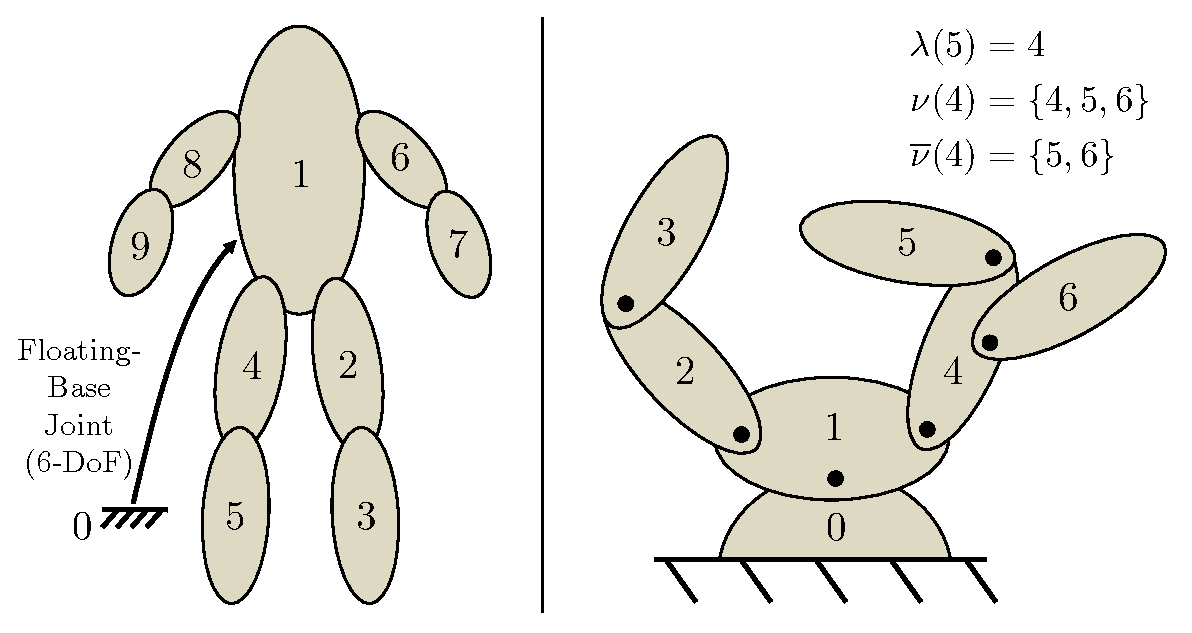
\includegraphics[width=.85 \columnwidth]{FloatFix.eps}
\caption{浮动和固定基座系统的机体编号和符号示例。}
\label{link_fig}
\end{figure}

\vspace{1ex}
\noindent {\bf 动力学:} 对于机体 $k$ 的空间运动方程~\cite{rbd} 给出为:
\begin{equation}
    \f_{k}= \I_{k}\a_{k} + \v_{k} \times^*\I_{k} \v_{k}
    \label{eq:spatial_eom}
\end{equation}
其中 $\f_{k}$ 是作用于机体 $k$ 的净空间力,$\I_{k}$ 是其空间惯量~\cite{rbd},并且 $\a_{k}$ 是其空间加速度。与将重力视为一个外力不同,一个常见的技巧是将基座向上加速,与重力加速度相反($\a_{0} = -\a_{g}$),提供机体 $k$ 的加速度为:
\begin{equation}
    \a_{k} = \textstyle\sum_{l \preceq k} \red{\big(} \red{\Phibar_{l}} \qdd_{l} + \v_{l} \times \red{\Phibar_{l}} \qd_{l} \red{\big)}+\a_{0}\,.
    \label{spatial_acc}
\end{equation}
%\noindent  %where, $\ag{k}$ is the spatial acceleration due to the gravity and is opposite of the gravity on body $i$ (i.e., $\ag{k} = -\a_{g} $). 
为了以后的使用,我们将 \red{$\a_k$} 分解为来自关节加速度的项,以及来自关节速率的项,根据
\[
 \gammabar_{k} = \textstyle \sum_{l \preceq k} \red{\Phibar_{l}} \qdd_{l}
\textrm{~~~and~~~}
\xibar_{k} = \textstyle \sum_{l \preceq k} \v_{l} \times \red{\Phibar_{l}} \qd_{l}  
\]
\red{($\gammabar, \xibar \in M^{6}$)}。根据这些定义, \red{$\a_k = \gammabar_k+\xibar_k + \a_{0}$}。


以类似方式,作用在机体 $k$ 上的净空间力分解为:
\begin{equation}
    \f_{k}=\etabar_{k} + \zetabar_{k}+\I_{k}\a_{0}
    \label{f_defn}
\end{equation}
其中,$\etabar_{k} = \I_{k} \gammabar_{k}$ \red{($\etabar \in F^{6}$)} 是关节加速度 $\qdd$ 引起的机体上的空间力,并且 $\zetabar_{k} = \v_{k} \times^{*}\I_{k} \v_{k} + \I_{k} \xibar_{k}$ ($\zetabar \red{\in F^{6}}$)  给出了机体 $k$ 上的科里奥利力和向心力。根据RNEA~\cite{rbd}的公式,$\red{\taubar_{i}} = \Phibar_{i}^{T}\f_{i}^{C} $,其中 $\f_{i}^{C}=\sum_{k \succeq i} \f_{k}$ 是通过关节 $i$ 传递的空间力。

\begin{figure*}[!b]
\hrulefill
\begin{align}
     \frac{\partial [\C\qd]_{i}}{\partial \red{\q_{j}}} = & \red{\Phibar_{i}^{T}  \Big[  2 \B_{i}^{C} \Psibardot_{j}  +     \I_{i}^{C} \v_{\lambda(j)}  \times \Psibardot_{j}   + } 
 \red{\I_{i}^{C} \xibar_{\lambda(j)} \times \Phibar_{j}  \Big] } 
     \label{CFO_q_eqn_1}
 \tag{26}\\
     \frac{\partial [\C\qd]_{j}}{\partial \red{\q_{i}}} = & \red{\Phibar_{j}^{T}  \Big[  2 \B_{i}^{C} \Psibardot_{i}  +     \I_{i}^{C} \v_{\lambda(i)} \times \Psibardot_{i} +}
     \red{\I_{i}^{C} \xibar_{\lambda(i)} \times \Phibar_{i}  + \zetabar_{i}^{C} \crff \Phibar_{i} \Big] , (j \neq i) }
    \label{CFO_q_eqn_2}
    \tag{27}
\end{align}
\end{figure*}


继续考虑系统整体,对于任意特定关节 $i$,方程(\red{\ref{inv_dyn}})可写成如下。

\begin{equation}
    \red{\taubar_{i}} =   [ \M(\q) \qdd]_{i}+   [\C(\q,\qd) \qd]_{i}  + \red{\g_{i}}(\q)
    \label{inv_dyn_expanded_eq2}
\end{equation}
%
则使用 $\red{\taubar_{i}}=\Phibar_{i}^{T}\f_{i}^{C} $,方程(\red{\ref{spatial_acc}}) 和 (\red{\ref{inv_dyn_expanded_eq2}}) 分解为: %the terms $[ \M(\q) \qdd]_{i}$, $[\C(\q,\qd) \qd]_{i}$, and $\g_{i}$ reduce to:
\begin{align}
 [\, \M(\q) \qdd \,]_{i} &= \red{\Phibar_{i}^{T}} \sum_{k \succeq i} [\I_{k} \gammabar_{k}]  
\label{mqdotdot_exp_2}\\[.5ex]
   [\,\C(\q,\qd) \qd\,]_{i} &= \red{\Phibar_{i}^{T}} \sum_{k \succeq i}[ \v_{k} \times^* \I_{k} \v_{k} + \I_{k}  \xibar_{k} ]
    \label{cqdot_exp_2}\\[.5ex]
    \red{\g_{i}} &=
   \red{ \Phibar_{i}^{T} \I_{i}^C  \a_{0}}
   \label{g_eqn}
\end{align}
其中, $\I{}_{i}^C$ 标志以机体 $i$ 为根的子树的复合刚体惯量,给出为 $\I{}_{i}^{C} = \sum_{k \succeq i} \I_{k}$。


\section{使用SVA解析偏导数}
\label{sec:fdsva}

在本节中,对于ID的导数推导出封闭形式表达式。对推导不太感兴趣的读者可以跳到方程(\ref{IDFO_SVA_eq1})和方程(\ref{Cqdot_FO_qdot_eqn})作为总结。



\newcommand{\qjp}[2]{q_{#1,#2}}

\subsection{构建矩阵块}
在附录~\ref{multi_dof_iden} 中给出了几个运动学特征式,作为主要推导的基础。
 \red{我们用 $n_j$ 标志关节 $j$ 的自由度数量。则对于该关节的运动子空间矩阵给出为
 $
 \Phibar_j = \begin{bmatrix} \phibar_{j,1} & \cdots \phibar_{j,n_j} \end{bmatrix}
 $
 其中,每一个空间向量 $\phibar_{j,p}$ 对于关节 $j$ 给出第 $p$ 个关节运动的自由模式。
 带一点符号随意,$\partial/ \partial \qjp{j}{p}$ 标志沿关节的这个第 $p$ 个关节的自由模式的方向导数的一个算子。例如,考虑到 $j \preceq i$ 的情况,给出特征式 J1:
 \begin{equation}
 \frac{\partial }{\partial \qjp{j}{p}} \Phibar_i = \phibar_{j,p}\times \Phibar_i \tag{J1}
 \end{equation}
 它提供了 $\Phibar_i$ 相对于在链中较早的关节 $j$ 处的相对运动 $\phibar_{j,p}$ 的变化率。对于旋转关节,这些导数只是常规的相对于关节角度的导数。用于多自由度关节如浮动基座,它们是更正式的李导数。 %For example, in a floating-base system when $j=1$ this formula would give the derivative of $\S_i$ with respect to rotation or translation along the $x$, $y$, and $z$ axes of the floating-base frame.
 %$q_{j,p}$ ($p \in n_{j}$) represents the $p^{th}$ element of the configuration space for the joint $j$. Corresponding to each $p$, $\phibar_{j,p}$ represents the joint motion axis vector of joint $j$ corresponding to the $p^{th}$ DoF. 
 %Considering the case when $j \preceq i$ (i.e., joint $j$ comes before joing $i$ in the tree), denote a directional deri have that:
% The identity J1 gives the rate of change of $\Phibar_{i}$ by perturbing the $p^{th}$ DoF of the joint $j$. 
考虑位形相关向量 $\boldsymbol{u}$,我们通过
\[
\frac{\partial \boldsymbol u}{\partial \q_j} = \Large \begin{bmatrix}\nicefrac{\partial \boldsymbol u}{\partial \qjp{j}{1}} & \cdots & \nicefrac{\partial \boldsymbol u}{\partial \qjp{j}{n_j}} \end{bmatrix}
\]
标志与关节 $j$ 相关的导数矩阵。为了说明,我们推导出特征式 J7,以便稍后在本节中使用。


%The identities J2-J9 are derived by perturbing DoFs pertaining to the full configuration space of the joint $j$. The identity J7 which is useful in the later section is derived as follows. 

考虑 $j \preceq i$ 并使用 $\gammabar_{i}$ 的定义:} 
\begin{equation}
    \frac{\partial \gammabar_{i}}{\partial \qjp{j}{p}} = \sum_{l \preceq i} \frac{\partial \Phibar_{l}}{\partial \qjp{j}{p}}  \qdd_{l}
    \label{dgamma_eq1}
\end{equation}
使用 J1 并交换叉积的顺序:

\begin{equation}
    \frac{\partial \gammabar_{i}}{\partial \qjp{j}{p}} = - \sum_{j \preceq l \preceq i} \Phibar_{l} \qdd_{l}  \times \phibar_{j,p}
\label{dgamma_eq3}
\end{equation}

\noindent 收集关节 $j$ 的所有自由度,方程(\ref{dgamma_eq3})变为:

\begin{equation}
    \frac{\partial \gammabar_{i}}{\partial \q_{j}} =  - \sum_{j \preceq l \preceq i} \Phibar_{l} \qdd_{l}  \times \Phibar_{j}
\label{dgamma_eq4}
\end{equation}

\noindent 使用 $\gammabar_{l}$ 的定义,对 $l$ 求和:

\begin{equation}
    \frac{\partial \gammabar_{i}}{\partial \q_{j}} = (\gammabar_{\lambda(j)} - \gammabar_{i}  )  \times \Phibar_{j}
\label{dgamma_eq5}
\end{equation}


\subsection{ID 相对于 $\q$ 的一阶偏导数}

\label{FO_ID_adsva_sec}

随后的推导使用这些公式和来自于附录 \ref{multi_dof_iden} 的特征式以获得在方程(\red{\ref{inv_dyn_expanded_eq2}})中的各项的偏导。由于推导过程相当冗长,因此本演示侧重于解释该方法。在附录~\ref{partials_details} 中提供完整的推导。

\vspace{1ex}
{\noindent \bf 方程(\red{\ref{mqdotdot_exp_2}})的偏导数:} 对于所有的 $ i,j \in \{1,\ldots,N\}$,我们推导 $[ \M(\q) \qdd]_{i}$ 相对于 \red{$\q_{j}$} 的偏导数。首先,考虑当 $j \preceq i$ 时的情况。使用在方程(\ref{mqdotdot_exp_2})中的微分的乘积规则:
  \begin{equation}
      \begin{aligned}
        \frac{\partial [ \M(\q)\qdd]_{i}}{\partial \q_{j}} = & \frac{\partial (\Phibar_{i}^{T})}{\partial \q_{j}} \sum_{k \succeq i} [\I_{k} \gammabar_{k}]   +  \\ &~~~    \Phibar_{i}^{T}  \sum_{k \succeq i} \Bigg[\frac{\partial \I_{k}}{\partial \q_{j}} \gammabar_{k} +  \I_{k} \frac{\partial \gammabar_{k}}{\partial \q_{j}} \Bigg]  
      \end{aligned}
\end{equation}
  对于项 $\frac{\partial (\Phibar_{i}^{T})}{\partial \q_{j}}$ 使用特征式 J3,对于项 $\frac{\partial \I_{k}}{\partial \q_{j}} \gammabar_{k}$ 使用特征式 J4,对于项 $\frac{\partial \gammabar_{k}}{\partial \q_{j}}$ 使用特征式 J7,并消除各项:
  
%   \begin{equation}
%       \begin{aligned}
%          \frac{\partial [ \M(\q) \qdd]_{i}}{\partial \q_{j}} = & -\Phibar_{i}^{T} \Big(\sum_{j \preceq i \preceq k} [\I_{k} \gammabar_{k}]  \crff \Big) \Phibar_{j}  +   \\ &
%          \Phibar_{i}^{T}  \sum_{j \preceq i \preceq k} \Bigg[(\I_{k} \gammabar_{k}) \crff \Phibar_{j} +  \I_{k}(\gammabar_{k} \times \Phibar_{j})+\\  &
%          \I_{k}  (\gammabar_{\lambda(j)} - \gammabar_{k}  )  \times \Phibar_{j} \Bigg]  
%       \end{aligned}
% \end{equation} 

  \begin{equation}
      \begin{aligned}
         \frac{\partial [ \M(\q) \qdd]_{i}}{\partial \q_{j}} =  &  \Phibar_{i}^{T}  \sum_{k \succeq i} \Big[
         \I_{k}  ( \gammabar_{\lambda(j)} \times ) \Big]   \Phibar_{j}
      \end{aligned}
\end{equation} 

\noindent 对索引 $k$ 求和后,最终表达式为:


\begin{equation}
      \frac{\partial [ \M(\q) \qdd]_{i}}{\partial \red{\q_{j}}} =  \red{\Phibar_{i}^{T} \Big[  \I_{i}^{C}  \gammabar_{\lambda(j)}   \times \Phibar_{j} \Big]} 
    \label{partial_Mqddot_1}
\end{equation}
对于 $i \red{\prec} j$ 的情况,我们有:
 \begin{equation}
         \frac{\partial [ \M(\q) \qdd]_{i}}{\partial \q_{j}} =   \Phibar_{i}^{T}  \sum_{k \succeq i} \Bigg[\frac{\partial \I_{k}}{\partial \q_{j}} \gammabar_{k} + \I_{k} \frac{\partial \gammabar_{k}}{\partial \q_{j}} \Bigg]
        \label{partial_Mqddot_4}
\end{equation}
 
\noindent 使用特征式 \red{J3、J4 和 J7} 并消除各项:
   \begin{equation}
      \begin{aligned}
       \frac{\partial [ \M(\q) \qdd]_{i}}{\partial \q_{j}} = 
     \Phibar_{i}^{T}  \sum_{ k \succeq j} \Big[(\I_{k} \gammabar_{k}) \crff + \I_{k}  (\gammabar_{\lambda(j)}  \times)  \Big]\Phibar_{j}  
        \label{partial_Mqddot_5}
      \end{aligned}
\end{equation} 

在索引 $k$ 上求和的结果为:

\begin{equation}
\frac{\partial [ \M(\q) \qdd]_{i}}{\partial \red{\q_{j}}} = \red{\Phibar_{i}^{T} \Big[\etabar_{j}^{C} \crff  + \I_{j}^{C} (\gammabar_{\lambda(j)} \times) \Big] \Phibar_{j}}
    \label{partial_Mqddot_2}
\end{equation}
其中,$\etabar_{j}^{C}$ 对于子树收集关节加速度相关的力,计算为 $\etabar_{j}^{C} = \sum_{k \succeq j} \etabar_{k}$。

为了便于实现,我们考虑一个单一情况,其中 $j \preceq i$。指数 $i$ 和 $j$ 在方程(\ref{partial_Mqddot_2})中被交换,以获取对于 $\frac{\partial [\M(\q)\qdd]_{j}}{\partial \q_{i}}$ 在\red{$j \prec i$}情况下的表达式。

\begin{align}
    & \frac{\partial [ \M(\q) \qdd]_{i}}{\partial \red{\q_{j}}} = \red{\Phibar_{i}^{T} \Big[  \I_{i}^{C}  \gammabar_{\lambda(j)}   \times \Phibar_{j} \Big]}  \label{Mqddot_FO_eqn} \\
    & \frac{\partial [ \M(\q)\qdd]_{j}}{\partial \red{\q_{i}}} = \red{\Phibar_{j}^{T} \Big[\etabar_{i}^{C} \crff + \I_{i}^{C} \gammabar_{\lambda(i)} \times  \Big] \Phibar_{i}, (j \neq i)} \nonumber
    %\end{aligned}    
\end{align}



\vspace{1ex}
{\noindent \bf 
方程(\red{\ref{cqdot_exp_2}})的偏导数:} 类似地,当 $j \preceq i$ 情况时,我们使用特征式 J2-J6 (附录 \ref{multi_dof_iden})以获得到 $[\C(\q,\qd) \qd]_{i}$ 相对于 \red{$\q_{j}$} 的一阶偏导数­,如方程(\ref{CFO_q_eqn_1},~\ref{CFO_q_eqn_2})所示。
\stepcounter{equation}
\stepcounter{equation}

 在这些方程中,对于子树,$\zetabar_{i}^C$ 的组合被定义为 $\zetabar{}_{i}^{C} = \sum_{k \succeq i} \zetabar_{k}$,并且矩阵 $\B_{k}(\v_{k},\I_{k})$ 是一个机体级别的科里奥利矩阵 \cite{nei_ms,nei_slotine,eche},给出为:
\begin{equation}
    \B_{k} = \frac{1}{2} \big[ \big(\v_{k}\times^* \big)\I_{k} - \I_{k} \big(\v_{k} \times   \big) + \big(\I_{k} \v_{k} \big) \crff    \big]
    \label{bl_term_defn}
\end{equation}
%
及其组合 $\B{}_i^C = \sum_{k\succeq i} \B_k$。

\vspace{1ex}
{\noindent \bf 重力项的偏导数:} \red{%Assuming the acceleration due to gravity $\ag{i}=-\ag{}$ on every body $i$ and 
使用特征式 J3 和 J4,} 对于 $j \preceq i$ 的情况,\red{$\g_{i}$} (方程~\ref{g_eqn}) 相对于 \red{$\q_{j}$} 的偏导数为:
\begin{equation}
    \begin{aligned}
         &  \frac{\partial \red{\g_{i}}}{ \partial \red{\q_{j}}} = \red{\Phibar_{i}^{T}  \I_{i}^{C}(\a_{0} \times \Phibar_{j})} \\
        & \frac{\partial \red{\g_{j}}}{ \partial \red{\q_{i}}} = \red{\Phibar_{j}^{T} \Big[(\I_{i}^{C}\a_{0})\crff + \I_{i}^{C}(\a_{0} \times ) \Big]\Phibar_{i} , (j \neq i)}
        \label{gFO_q_eqn}
    \end{aligned}
\end{equation}



\noindent {\bf ID相对于$\q$的各偏导的摘要:} 单个组件的偏导现在被收集在一起。

\noindent 将在方程(\ref{Mqddot_FO_eqn})、(\ref{CFO_q_eqn_1})、(\ref{CFO_q_eqn_2})和(\ref{gFO_q_eqn})中的各项相加,以获得在 $j \preceq i$ 情况下对于 $\frac{\partial \taubar}{\partial \q}$ 的总表达式。在附录~\ref{combine_terms} 中提供完整的推导。

% modified
\begin{align}
    %\begin{aligned}
        \frac{\partial \red{\taubar_{i}}}{\partial \red{\q_{j}}} = & \red{ \Phibar_{i}^{T} \big[ 2  \B_{i}^{C} \big] \Psibardot{}_{j} + \Phibar_{i}^{T}  \I_{i}^{C} \Psibarddot{}_{j} } \label{IDFO_SVA_eq1} \\
        \frac{\partial \red{\taubar_{j}}}{\partial \red{\q_{i}}} = & \red{\Phibar_{j}^{T} [ 2 \B_{i}^{C} \Psibardot_{i} +  \I_{i}^{C}  \Psibarddot_{i}+(\f_{i}^{C} )\crff \Phibar_{i}  ] (j \neq i)} \nonumber
    %\end{aligned}
\end{align}
%The quantity $\f{}_{i}^{C}$ is the composite force $\f$ on the sub-tree at body $i$, defined as $\f{}_{i}^{C} = \sum_{l \succeq i} \f_{l}$. 
\red{该空间量 $\Psibardot_{j}$ 和 $\Psibarddot_{j}$ 被定义为:}

\begin{align}
\begin{split}
  \red{\Psibardot_{j} = }& \red{\v_{\lambda(j)} \times \Phibar_j} \\
\red{ \Psibarddot_{j} = }& \red{\a_{\lambda(j)} \times \Phibar_{j} + \v_{\lambda(j)} \times \Psibardot_{j}}
\end{split}
\label{psidot_psidotdot_defn}
\end{align}


\subsection{ID 相对于 $\qd$ 的一阶偏导数}

$\taubar$ 相对于 $\qd$ 的偏导\red{仅依赖于科里奥利项 $\C \qd$}。使用特征式J8和J9导致当 $j \preceq i$ 情况时的表达式(参见附录~\ref{partials_qd} 的完整推导):

\begin{equation}
    \begin{aligned}
    & \frac{\partial \red{\taubar_{i}}}{\partial \red{\dot{\q}_{j}}} =\frac{\partial [\C  \qd]_{i}}{ \partial \red{\dot{\q}_{j}}} = \red{\Phibar_{i}^{T} \Big[2 \B_{i}^{C} \Phibar_{j} +  \I_{i}^{C} (    \Psibardot_{j} + \Phibardot_{j} ) \Big]  }\\
    & \frac{\partial \red{\taubar_{j}}}{\partial \red{\dot{\q}_{i}}} =\frac{\partial [\C  \qd]_{j}}{ \partial \red{\dot{\q}_{i}}} = \red{\Phibar_{j}^{T} \Big[2 \B_{i}^{C} \Phibar_{i} +  \I_{i}^{C} (    \Psibardot_{i} + \Phibardot_{i} ) \Big]  (j \neq i)}
\label{Cqdot_FO_qdot_eqn}
    \end{aligned}
\end{equation}

\subsection{ID的一阶偏导算法}
算法 \ref{alg:tau_FO_v2} 返回在方程(\red{\ref{IDFO_SVA_eq1}})和方程(\red{\ref{Cqdot_FO_qdot_eqn}})中的各项,并具有计算复杂度 $\mathcal{O}(Nd)$。该方法与以地面帧坐标表达的所有空间向量一起计算。
第一遍是在前向方向,并从根部到叶子节点计算空间速度,加速度,$\Phibardot_{i}$,$\Psibardot_{i}$,$\Psibarddot_{i}$,$\B_{i}$,以及空间力 $\f_{i}$。当关节 $i$ 具有一个单一自由度时,$\Phibardot_i = \Psibardot_i$ 并且 $\ddot{\Phibar}_i =\Psibarddot_{i}$ 而且计算步骤与文献 \cite[Alg.~2]{jain} 中的相同。

第二遍是后向方向,从叶子节点到根部。索引$i$获取从$1$到 $N$ 的所有值。该量 $\frac{\partial \boldsymbol\tau}{\partial \q}[\subtree(i), i]$ 标志 $\boldsymbol\tau$ 对于在 $i$ 的子树中所有机体相对于 $\q_{i}$ 的偏导数,而 $\frac{\partial \boldsymbol\tau}{\partial \q}[i, \subtreeb(i)]$ 是 $\boldsymbol\tau$ 对于机体 $i$ 相对于在 $i$ 的子树中每一个机体的偏导数,不包括机体 $i$。 %The composite quantities $\I_i^{C}$, $\B_i^{C}$, and $\f_i^{C}$ are calculated recursively for each sub-tree.  
该后向遍历再次推广了在文献 \cite[Alg.~2]{jain} 中的一个算法。区别是,第15行的第三项在单一自由度情况可以被丢弃(因为在这种情况下 $ {\Phibar}_i^T (\f_i^C \crff) {\Phibar}_i =0$)。而第17-20行重组在文献 \cite{jain} 中的第二层内循环为矩阵乘法。
%Common terms like $\B_{i}^{C}$ and $\big( \I_{i}^{C} \red{\Phibar_{i}} \big)$ in Eq.\red{~\ref{IDFO_SVA_eq1}} and Eq.\red{~\ref{Cqdot_FO_qdot_eqn}} are evaluated only once and re-used to build an efficient algorithm.
% The final form of the algorithm is found to bear a great deal of resemblance to Algorithm 2 in \cite{jain}, however, the derivation here is tailored for branched trees, further optimized as considered in the next section, and compared with chain-rule approaches for the first time.


\begin{algorithm}[t]
\small
\caption{IDSVA 算法}
%\begin{multicols}{2}

\begin{algorithmic}[1]  % this [1] is used to number the lines of the algorithm
%\begin{algorithmic}
\REQUIRE $ \q, \,\qd ,\, \qdd,\, model$

\STATE $ \v_0 = 0; \, \a_{{0}} = -\a_g  $
%STATE $  $
%\STATE $$
%\STATE $ $

\FOR{$i=1$ to $N$}

%\red{\STATE  $ \vJ{i} =   \Phibar_{i}  \qd_{i}$}

\STATE  $ \v_{i} =  \v_{\lambda(i)} +  \red{\Phibar_i} \qd_{i}$

%\red{\STATE  $ \aJ{i} =  \Phibar_i \ddot{\q}_{i} + \v_i \times \Phibar_{i} \qd_i$}

\STATE $\a_{i} =  \a_{\lambda(i)} +  \Phibar_i \ddot{\q}_{i} + \v_i \times \Phibar_{i} \qd_i$ \\

\STATE $ \red{\Phibardot_i}  =  \v_{i} \times \red{\Phibar_i}  $\\[.5ex] 

\red{\STATE $\Psibardot_i  =  \v_{\lambda(i)}\times \Phibar_i  $\\[.5ex] 

\STATE $\Psibarddot_i  =  \a_{\lambda(i)}\times \Phibar_i + \v_{\lambda(i)}\times \Psibardot_i   $ \\[.5ex]

}

\STATE $\I_i^C = \I_i$
\STATE $ \B_i^C = \frac{1}{2}[ ( \v_{i} \times^*) \I_i -  \I_i  ( \v_{i} \times ) + (\I_i \v_i )\crff ]  $\\[.5ex]

\STATE $ \f_i^C =  \I_i  \a_{i} + ( \v_{i} \times^*) \I_i \v_{i}  $\\[.5ex]  % 6x1 vector


\ENDFOR

% Second Loop starts here

\FOR{$i=N$ to $1$}

\STATE $ \t_1[i] = \I{}_{i}^C  \red{{\Phibar}_i} $\\[.5ex] % t2 6x1 vector

\STATE $\t_2[i] = 2\B{}_i^C \red{\Phibar_i} + \I_i^C ( \red{\Phibardot_i + \Psibardot_i } )$\\[.5ex] % T4 6x6 matrix

 \STATE $\t_3[i] = 2 \B{}_i^C  \red{\Psibardot_i} + \I{}_{i}^C \red{\Psibarddot_i}  + \red{\f_i^C \crff {\Phibar}_i}  $\\[.5ex]
\STATE $\t_4[i] =   2[\B_i^C]\T \red{{\Phibar}_i}$\\[.5ex] % 6x1 vector

\STATE $\frac{\partial \boldsymbol\tau}{\partial \q}[i, \subtreeb(i)] = \Phibar_i\T \t_3[\subtreeb(i)]$ \\[1ex]

\STATE $\frac{\partial \boldsymbol\tau}{\partial \qd}[i, \subtreeb(i)] = \Phibar_i\T \t_2[\subtreeb(i)]$ \\[1ex]


\STATE $\frac{\partial \boldsymbol\tau}{\partial \q}[\subtree(i), i] =\t_4[\subtree(i)]\T \Psibardot_i +  \t_1[\subtree(i)]\T \Psibarddot_i $ \\[1ex]


\STATE $\frac{\partial \boldsymbol\tau}{\partial \qd}[ \subtree(i), i] = \t_4[\subtree(i)]\T \Phibar_i + \t_1[\subtree(i)]\T (\Phibardot_i + \Psibardot_i) $ \\[1ex]


    \IF {$\lambda(i) > 0$}
    
        \STATE $\I_{\lambda(i)}^C = \I_{\lambda(i)}^C + \I_i^C ; \, \B_{\lambda(i)}^C = \B_{\lambda(i)}^C +  \B_i^C $ \\[.5ex]
        \STATE $ \f_{\lambda(i)}^C = \f_{\lambda(i)}^C +  \f_i^C $ 

    \ENDIF

\ENDFOR
\RETURN $\frac{\partial \taubar }{\partial{\q}},\frac{\partial \taubar }{\partial{\qd}}$

\end{algorithmic}
%\end{multicols}

\label{alg:tau_FO_v2}
\end{algorithm}



%\section{Implementation Considerations}
%\label{sec:efficient_SVA}

\subsection{FD与ID的相关偏导}
\label{sec:efficient_SVA}

方程(\ref{car_FO_eqn})给出FD和ID的导数之间的关系,其中 $\frac{\partial ID }{\partial \u}$ ($\u = [\q, \qd ]$) 是一个 $n \times 2n$ 矩阵,并且 $\M^{-1}$ 是一个 $n \times n$ 矩阵。两个矩阵直接相乘的结果产生一个 $\mathcal{O}(N^3)$ 计算,且它被称为直接矩阵相乘(Direct Matrix Multiplication, DMM)。一种具有计算复杂度为 ($\mathcal{O}(N^2)$) 的替代方法 
%to calculate the product of $\M^{-1}$ with $\frac{\partial ID }{\partial \u}$
将在本节中介绍。

对于一个给定的 $\taubar$,ABA给出了 $\qdd$ (方程~\ref{fwd_dyn2}),表示为:
\begin{equation}
       \qdd = ABA(\q,\qd,\taubar,\a_g)
    \label{ABA_eqn_1}
\end{equation}
%
根据方程(\ref{fwd_dyn2}),对于 $\qd=\bf{0}$, $\a_g=\bf{0}$ 和一个任意输入向量 $\taubar=\b$,
%\begin{equation}
$
     \qdd = \M^{-1} \b
    \label{fwd_dyn3}
    $。
%\end{equation}
矩阵 $\M^{-1}$ 与任意向量 $\b$ 的乘积因此可被计算为: %using ABA with $\qd=\bf{0}$, $\a_g=\bf{0}$, and input vector $\b$:
\begin{equation}
       \M^{-1} \b  = ABA(\q,\bf{0},\b, \bf{0})
    \label{ABA_eqn_2}
\end{equation}
对于 $\M^{-1}$ 与任意给定的矩阵(大小为$n \times m$)的乘积,ABA可以使用$m$次,其中$\qd=\bf{0}$,$\a_g=\bf{0}$ 和 $\b$ 做为给定矩阵的列向量,一次使用一个,其结果产生一个 $\mathcal{O}(Nm)$ 运算。由于对于每一个输入列向量重复使用ABA,运动学变量和铰接惯量仅计算一次,并被保存以供重复使用。为实现方程(\ref{car_FO_eqn}),方程(\red{~\ref{ABA_eqn_2}}) 与做为 $\frac{\partial ID }{\partial \u}$ 的列向量 $\b$ 一起被使用,一次一个。该过程被定义为“ABA-零算法” (ABA-Zero-Algorithm, AZA),因为输入 $\qd$ 和 $\a_g$ 都为 $\bf{0}$。

\section{结果}

\subsection{算法正确性}
 将来自ABACR、FDSVA和FDCR的FD偏导数与在一个Fortran实现中的使用复杂步长法计算的导数进行比较,以确定其精确度。对于 $N=100$,ABACR方法会导致逐项的均方根(root-mean-square, rms)相对误差为 $10^{-13}$,而FDSVA和FDCR两者的均方根误差约为 $10^{-12}$。所有方法的均方根相对误差在对数尺度上随自由度的增长而线性增长。 %Further accuracy analyses of the partial derivatives will be provided in future work.
 

\subsection{ID/FD与RNEACR/FDCR偏导的运行时间对比,如文献\cite{car}所示,通过Fortran实现两者}

我们考虑一个有 $N$ 个连杆的串联或\red{分支}运动学树,所有的旋转关节都可围绕它们的局部 $z$ 轴旋转。

在机体座标上的RNEACR\cite[Algos.~2 \& 3]{car} (表~\ref{table2}) 被用于计算ID的偏导数,并与IDSVA (表~\ref{table2}) 方法进行比较。所有的算法都用Fortran 90编写,并使用Intel Fortran编译器在一台3.07 GHz Intel Xeon处理器上实现。为了计算平均运行时间,在状态变量和控制变量为随机输入的情况下,每个算法运行 10,000 次。图~\ref{all_plots_fortran} 显示了两种方法的比较。对于$N=100$,发现IDSVA速度提高比RNEACR快 $15 \times$ 倍。

 图~\ref{all_plots_fortran} 还显示了对于串联链的FDSVA与FDCR和ABACR的比较 (表~\ref{table2})。使用本文开发的解析导数表达式,FDSVA方法对于所有的 $N \ge 2$ 的值上都优于FDCR。
 
 \blue{由于SVA允许坐标自由的表达式,递归算法可以在机体坐标或地面坐标中制定~\cite{rbd}。对于机体坐标算法,所有中间量都使用变换矩阵 $\prescript{i}{}{\boldsymbol{X}}_{\lambda(i)}$在机体坐标之间进行变换,而对于地面坐标算法,这些中间量可以保留地面帧形式。后者的一个主要优点是避免了在算法的后向遍历中局部机体帧之间的重复变换。此增益是在外向遍历期间以地面坐标帧表示运动学量(速度 $\prescript{0}{}{\v}_{i}$、加速度 $\prescript{0}{}{\a}_{i}$)、关节运动子空间矩阵  $\prescript{0}{}{\Phibar}_{i}$,以及惯量矩阵 $\prescript{0}{}{\I}_{i}$ 为代价实现的。图~\ref{idsva_bf_vs_gf} 显示了在机体坐标和地面坐标下IDSVA (参见表~\ref{table2}) 的运行时间的比较。对于 $N=2$ 到 $N=500$,地面坐标算法的加速比在1.3到1.9之间。 % The ground coordinates algorithm is moderately faster due to avoiding repeated transformations on the  $\t_1,\ldots,\t_4$ variables in the backward pass.
 }
 
 
 
\begin{figure}[tb]
\hspace{-0.5cm}
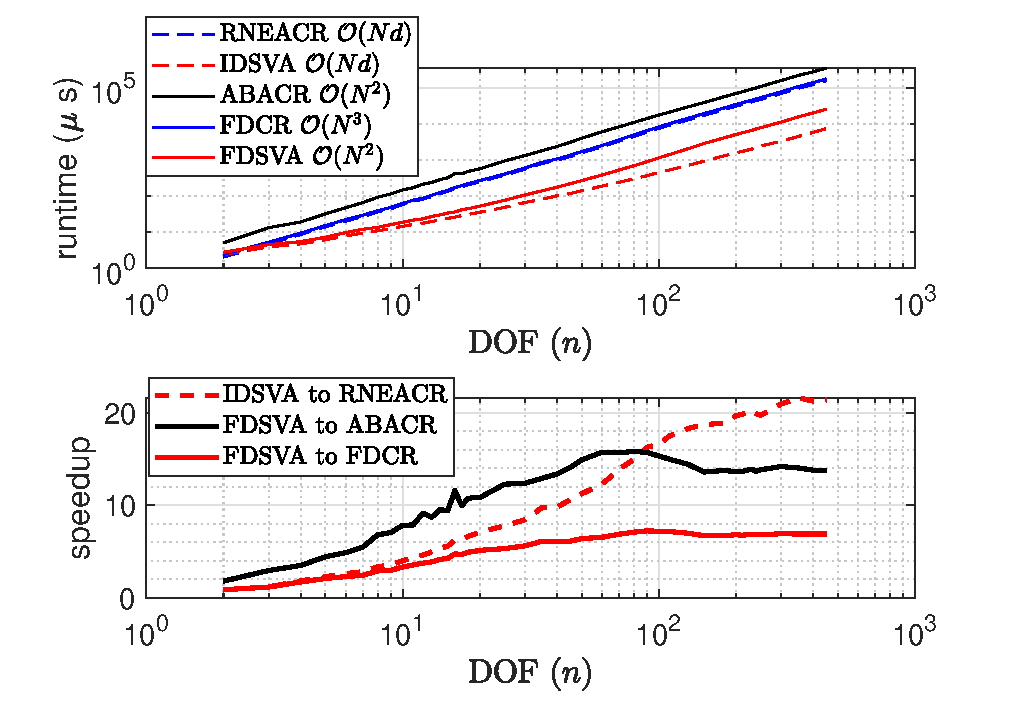
\includegraphics[width=9cm]{all_plots_fortran.eps}
\caption{IDSVA的Fortran实现优于RNEACR,FDSVA的优于FDCR和ABACR (表~\ref{table2}),适用于所有 $N \succeq 2$ 的串联链(对于旋转关节,$N = n$)}
\label{all_plots_fortran}
\end{figure}


\begin{figure}[tb]
\hspace{-0.5cm}
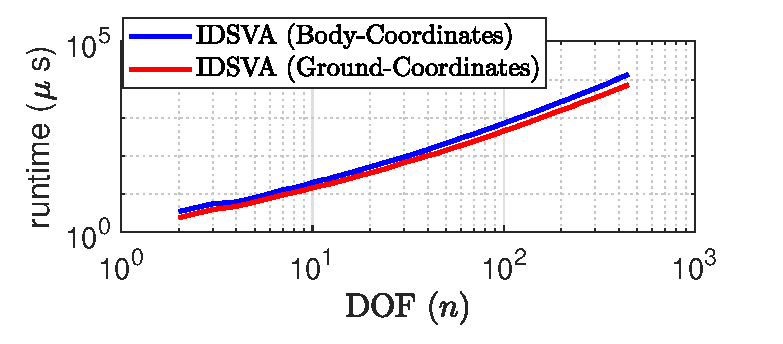
\includegraphics[width=9cm]{IDSVA_bf_vs_gf.eps}
\caption{\blue{IDSVA在地面与机体坐标帧中的Fortran实现。}}
\label{idsva_bf_vs_gf}
\end{figure}


\begin{figure}[tb]
%\hspace{-0.5cm}
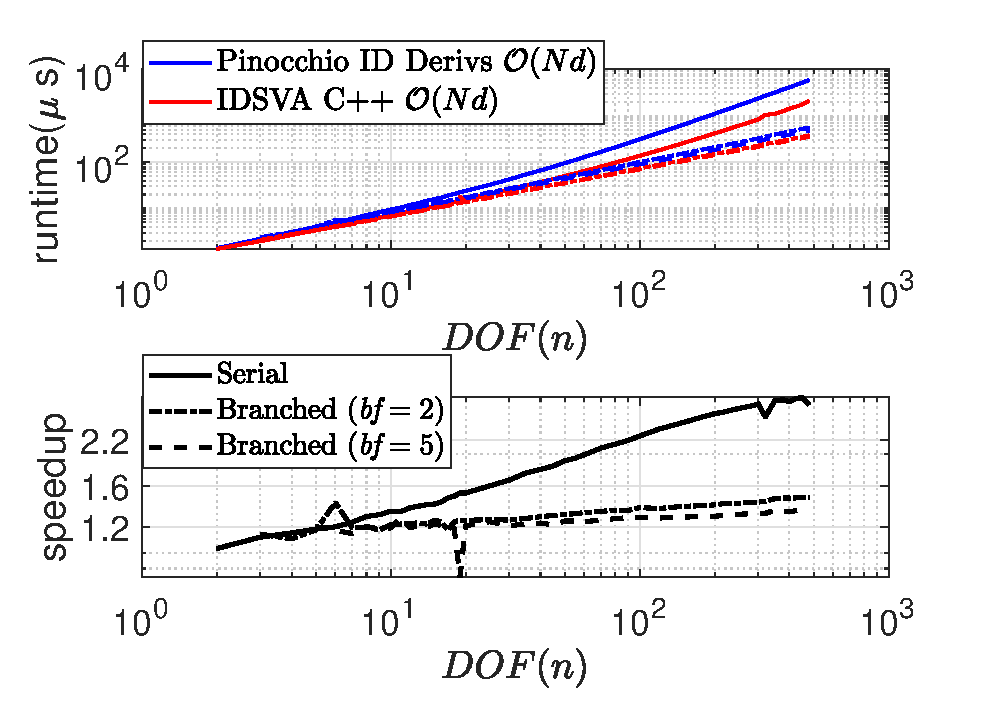
\includegraphics[width=9cm]{rneacr_vs_idsva_gcc_wo_march.eps}
\caption{a) 串联链(实线)、分支链(\textit{bf}=2,虚线)、分支链条(\textit{bf}=5,虚线) b) IDSVA C++ 对于所有的 $N \geq 2$ 的Pinocchio ID Derivs的改进 (gcc-9.0编译器)。对于具有旋转关节的运动学树,$N = n$。}
\label{SVA_vs_RNEA_FO_fig}
\end{figure}




\subsection{ID/FD的C++偏导的运行时间与附带于文献\cite{car}的Pinocchio实现的对比}
地面坐标中的IDSVA在Pinochho框架内用C++实现。该策略可以直接与Pinochhio的原始ID偏导数进行比较~\cite{car_code}。图~\ref{SVA_vs_RNEA_FO_fig} 显示了具有一些分支因子 \textit{bf} ~\cite{rbd}的串联和分支运动学树的两种方法的比较。对于 $N=100$ 的串联链,使用gcc-9.0编译器和关闭turbo boost可以获得 $2 \times$ 倍的加速。图~\ref{pin_comparison} 显示了使用LLVM Clang-10和gcc-9.0编译程序将IDSVA C++实现到多自由度关节机器人的结果。对于50个连杆的浮动基座仿人机器人Talos,IDSVA使用gcc-9.0编译器,其速度比Pinocchio \cite{car_code} 中的Pinocchio ID Derivs算法快 $1.4 \times$ 倍。Pinocchio ID Derivs (开源,但未公开)和IDSVA之间有一个基本的相似之处。这两种算法基本上都计算相同的量,但IDSVA C++中更高效的后向遍历重组导致了图~\ref{pin_comparison} 所示的加速。与Pinocchio ID Derivs代码中机体 $i$ 的祖先上的 $\mathcal{O}(d)$ 最内层第二遍后向遍历相比,IDSVA在第19行和第20行对机体 $i$ 的子树使用矩阵-矩阵乘法,从而提高速度。这一小小的改变使Pinocchio的性能达到了最先进的水平,并被纳入了最新的版本中。图~\ref{fdsva_fdcr_pin} 显示了FDSVA C++ (在Pinocchio中实现) 的CPU运行时间与Pinocchio FD Derivs的串联和分支运动树的比较。IDSVA的开源Pinocchio实现参见文献 \cite{cppsource},以及MATLAB版本参见文献 \cite{matlabsource}。
 
\begin{figure}[tb]
\hspace{-0.5cm}
\center
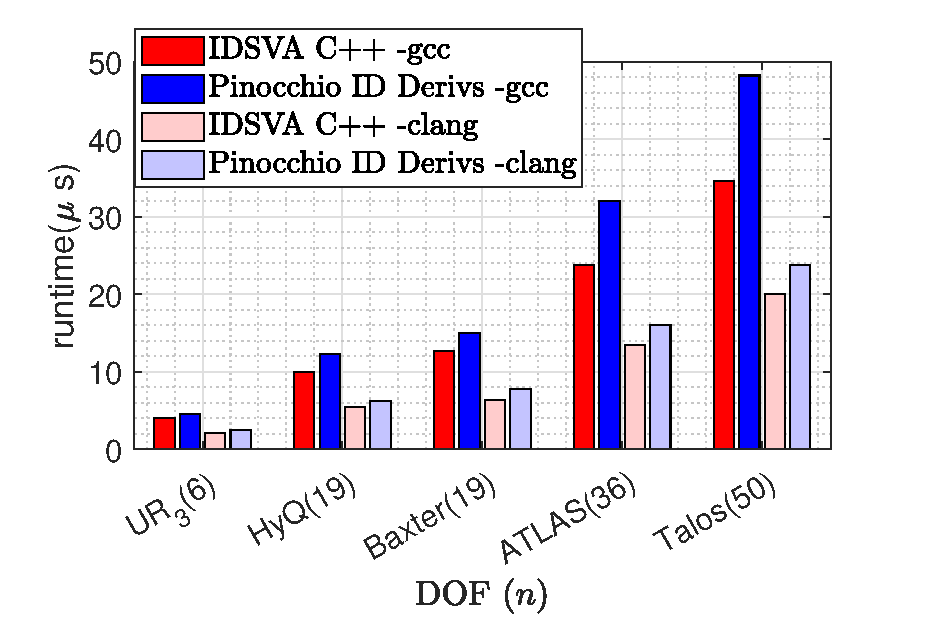
\includegraphics[width=8.5cm]{rneacr_vs_idsva_bar_clang_gcc_ral_w_march_ral.eps}
\caption{\red{几种浮动基座多自由度机器人的IDSVA (在 C++ 中) 与Pinocchio ID Derivs~\cite{car_code} 框架的比较($n$)固定基座 UR3,Baxter。使用gcc-9.0编译器(深红/蓝色)、LLVM Clang-10编译器(浅红色/蓝色)的浮动基座 HyQ、ATLAS、Talos。$N \neq n$,适用于具有多自由度关节的模型。} }
\label{pin_comparison}
\end{figure}


% original
\begin{figure}[tb]
\hspace*{-0.5cm}
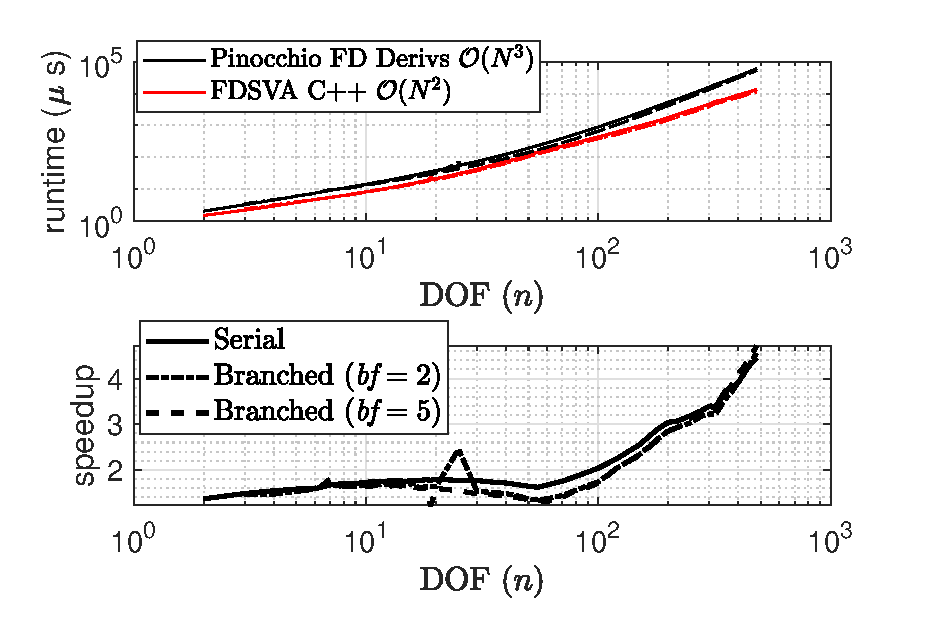
\includegraphics[width=9cm]{fdcr_vs_fdsva_wo_march_gcc.eps}
\caption{a) 对于串联和分支树的FD的一阶偏导数,Pinocchio FD Derivs与FDSVA C++的CPU运行时间比较(对于旋转关节,$N=n$)。串联链(实线)、分支链(\textit{bf}=2,虚线)、分支链条(\textit{bf}=5,虚线) b) 加速图显示FDSVA C++ 对于所有的$N$,都优于Pinocchio FD Derivs。}
\label{fdsva_fdcr_pin}
\end{figure}

\subsection{在C++中AZA的CPU运行时间与附带于文献\cite{car}的Pinocchio实现的DMM的比较}
AZA在 Pinocchio~\cite{car_code} 框架中实现。Pinocchio的 $\M^{-1}$ 算法~\cite{InverseMassMatrix} 被修改为包括AZA。在图~\ref{dmm_vs_aza} 中,“交叉点” $N$ 标志DMM比AZA表现得更好的点。该点取决于用于实现算法的硬件和编译器优化设置,但对于较高的 $N$,$\mathcal{O}(N^2)$ AZA是高效的,因为它避免了昂贵的矩阵-矩阵乘法。表~\ref{table_ipr} 给出了交叉点的 $N$ 值(对于运动学树),在不同编译器设置下,AZA的性能优于DMM。这种交叉点的 $N$ 的影响可以在图~\ref{fdsva_fdcr_pin} 中看到,对于 $N=50$ 的FDSVA曲线,由于从DMM切换到AZA,算法的秩从 $\mathcal{O}(N^3)$ 变为 $\mathcal{O}(N^2)$ ,从而得到方程(\ref{car_FO_eqn})。

\begin{figure}[tb]
%\hspace{0.5cm}
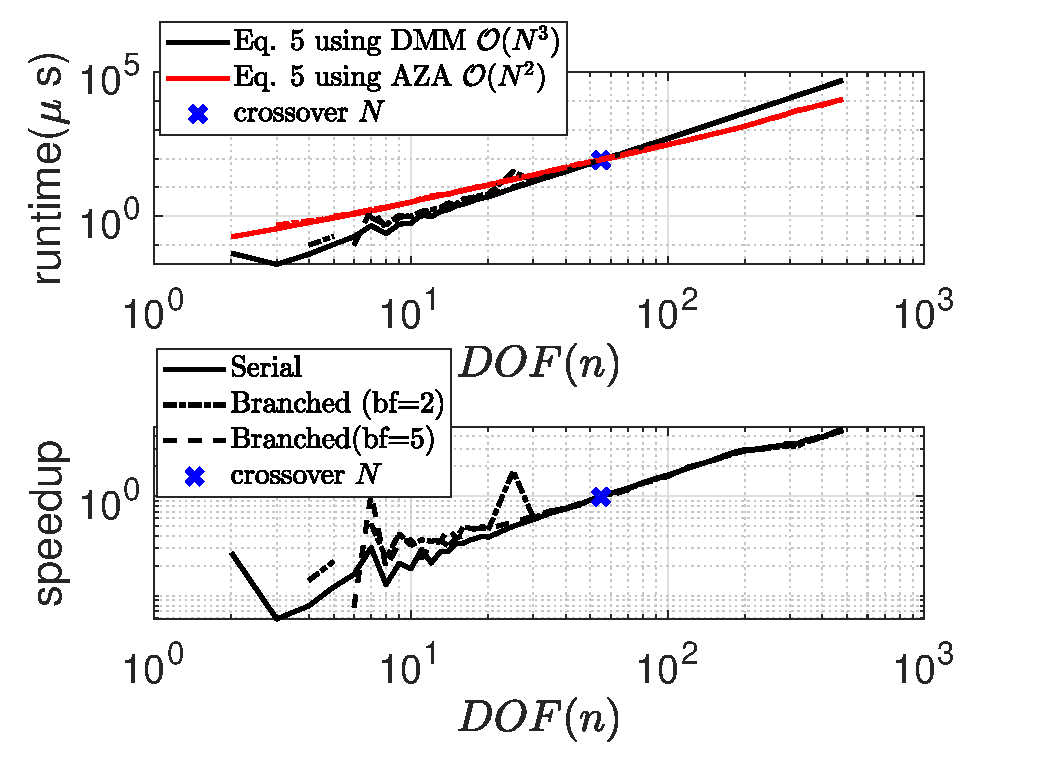
\includegraphics[width=8.5cm]{DMM_vs_AZA_pinocchio.eps}
\caption{a) 在Pinocchio C++框架中实现的DMM与AZA运行时间的比较(使用gcc-9.0)显示了串联链(实线)、分支链(\textit{bf}=2,虚线)和分支链(\textit{bf}=5,虚线)在50处的交叉点 $N$。 b) 在对数-对数尺度上,AZA相对DMM的速度随着 $n$ 的线性增长而增长,对于具有旋转关节的运动学树,$N=n$。}
\label{dmm_vs_aza}
\end{figure}

\begin{table}[tb]
\centering
\begin{tabular}{ |c|c|c| } 
 \hline
 Compiler & AVX Off & AVX On \\ 
  \hline
 gcc-9.0 & 50 & 450 \\ 
 clang-10 & 80 & 350 \\ 
 \hline
\end{tabular}
 \caption{使用不同的编译器和自动矢量化 (\texttt{march=native}) 设置的交叉点 $N$ (自由度)。}
  \label{table_ipr}
\end{table}

 


%\vspace{-0.5cm}


\section{实现考虑事项}
\label{sec:efficient_SVA}



\section{结论}
在本项工作中,我们提出了逆动力学的封闭形式的偏导数,以及一个高效的算法,以计算具有多自由度关节和浮动基座的机器人的逆动力学和正向动力学部分。以优化算法的在线和离线应用。一些算法的优化和空间向量代数(Spatial Vector Algebra, SVA)的特征被利用以使能高效的实现。该方法使用gcc编译器为TALOS人形模型提供了$1.4 \times$倍于最先进的Pinocchio FD导数的加速,并且使用Clang-10编译器提供了$1.2 \times$倍的加速。偏导数运行时间的减少使得在线和离线应用程序的优化算法更快。这些改进的时序最终可以导致腿式和工业机器人有更好的运动规划。


\section{Acknowledgement}
This work was partially supported by the National Science Foundation EAGER grant CMMI-1835013. The authors thank Pinocchio developers Justin Carpentier \& Nicolas Mansard for important feedback and Wolfgang Merkt for benchmarking the IDSVA algorithm.

% This is working !
%\bibliographystyle{IEEEtran}
%\bibliographystyle{unsrt}
%\bibliography{main.bib}

\begin{thebibliography}{99}

\bibitem{neunert}
M. Neunert et al., "Whole-Body Nonlinear Model Predictive Control Through Contacts for Quadrupeds," in \textit{IEEE Robotics and Automation Letters}, vol. 3, no. 3, pp. 1458-1465, 2018. %doi: 10.1109/LRA.2018.2800124.

\bibitem{posa}
 M. Posa, C. Cantu, R. Tedrake , "A direct method for trajectory optimization of rigid bodies through contact," \textit{The International Journal of Robotics Research}, vol. 33, no. 1, pp. 69-81, 2014. %doi:10.1177/0278364913506757
  
\bibitem{crocoddyl}
C. Mastalli, R. Budhiraja, W. Merkt, G. Saurel, B. Hammoud, et al, "Crocoddyl: An Efficient and Versatile Framework for Multi-Contact Optimal Control," in
\textit{IEEE Int.~Conf.~on Robotics and Automation}, 2020.

\bibitem{drake}
R. Tedrake and the Drake Development Team, "Drake: Model-based design and verification for robotics" 2019, url - https://drake.mit.edu.

\bibitem{car}
J. Carpentier, N. Mansard, "Analytical Derivatives of Rigid-Body Dynamics Algorithms," in \textit{Robotics: Science and Systems},  Pittsburgh, United States, Jun. 2018.

\bibitem{car_code}
\red{\textit{Pinocchio} (2.6.0). Inria. [Online]. Available: \url{https://github.com/stack-of-tasks/pinocchio/releases/tag/v2.6.0}}

  \bibitem{mujoco}
E. Todorov, T. Erez and Y. Tassa, "MuJoCo: A physics engine for model-based control," in \textit{IEEE/RSJ Int.~Conf.~ on Intelligent Robots and Systems}, 2012, pp. 5026-5033. %doi: 10.1109/IROS.2012.6386109



\bibitem{tassa}
Y. Tassa, T. Erez and E. Todorov, "Synthesis and stabilization of complex behaviors through online trajectory optimization," in \textit{IEEE/RSJ Int.~Conf.~on Intelligent Robots and Systems}, 2012, pp. 4906-4913. %doi: 10.1109/IROS.2012.6386025.

\bibitem{koena}
J. Koenemann et al., "Whole-body model-predictive control applied to the HRP-2 humanoid," in \textit{IEEE/RSJ Int.~Conf.~on Intelligent Robots and Systems}, 2015, pp. 3346-3351. %doi: 10.1109/IROS.2015.7353843.

\bibitem{Kudruss}
M. Kudruss, P. Manns and C. Kirches, "Efficient derivative evaluation for rigid-body dynamics based on recursive algorithms subject to kinematic and loop constraints," \textit{IEEE Control Systems Letters}, vol. 3, no. 3, pp. 619-624, 2019. %doi: 10.1109/LCSYS.2019.2914338.

\bibitem{robcogen}
M. Giftthaler, M. Neunert, M. Stäuble, M. Frigerio, C. Semini, and J. Buchli, "Automatic differentiation of rigid-body dynamics for optimal control and estimation," \textit{Advanced Robotics}, vol. 31, no. 22, pp. 1225-1237, 2017. %doi:10.1080/01691864.2017.1395361

\bibitem{cstep}
J.N. Lyness, and C. B. Moler, "Numerical differentiation of analytic functions," \textit{SIAM Journal on Numerical Analysis}, vol. 4, no.2, 202-210, 1967.

\bibitem{complex}
C. C. Cossette, A. Walsh and J. R. Forbes, "The Complex-Step Derivative Approximation on Matrix Lie Groups," \textit{IEEE Robotics and Automation Letters}, vol. 5, no. 2, pp. 906-913, 2020. %doi: 10.1109/LRA.2020.2965882.

\bibitem{mcx}
\red{G. Lantoine, R. Russell and T. Dargent, "Using Multicomplex Variables for Automatic Computation of High-Order Derivatives," \textit{ACM Trans. Math. Softw.},38, 3, Article 16 (April 2012). }

\bibitem{sohl2001recursive}
G.~A. Sohl and J.~E. Bobrow, ``A recursive multibody dynamics and sensitivity
  algorithm for branched kinematic chains,'' \emph{J. Dyn. Sys., Meas.,
  Control}, vol. 123, no.~3, pp. 391--399, 2001.
  
  
\bibitem{lee2005newton}
\red{S.-H. Lee, J.~Kim, F.~C. Park, M.~Kim, and J.~E. Bobrow, ``Newton-type
  algorithms for dynamics-based robot movement optimization,'' \emph{IEEE
  Trans.~on Robotics}, vol.~21, no.~4, pp. 657--667, 2005.}

\bibitem{garofalo}
G. Garofalo, C. Ott and A. Albu-Schäffer, "On the closed form computation of the dynamic matrices and their differentiations," in \textit{IEEE/RSJ Int.~Conf.~on Intelligent Robots and Systems}, 2013, pp. 2364-2359. %doi: 10.1109/IROS.2013.6696688.

\bibitem{jain}
  A. Jain and G. Rodriguez, “Linearization of manipulator dynamics using spatial operators,” \textit{IEEE Trans.~on Systems, Man, and Cybernetics}, vol. 23, no. 1, pp. 239–248, 1993. 


\bibitem{rbd}
R. Featherstone, \textit{Rigid-Body Dynamics Algorithms},
Springer, 2008.


\bibitem{eche}
\red{S. Echeandia, and P. M. Wensing,  "Numerical Methods to Compute the Coriolis Matrix and Christoffel Symbols for Rigid-Body Systems." ASME. J. Comput. Nonlinear Dynam. September 2021; 16(9): 091004. }

\bibitem{nei_ms}
G. D. Niemeyer, "Computational Algorithms for Adaptive Robot Control", Master's thesis, MIT, Boston, 1990.

\bibitem{nei_slotine}
G. Niemeyer, J.-J. E. Slotine "Performance in Adaptive Manipulator Control," \textit{The International Journal of Robotics Research}, vol 10, no. 2, pp 149-161, 1991.

\bibitem{cppsource}
\red{\url{https://github.com/shubhamsingh91/pinocchio}}

\bibitem{matlabsource}
\red{\url{https://github.com/ROAM-Lab-ND/spatial_v2_extended}}

\bibitem{InverseMassMatrix}
\red{J. Carpentier, "Analytical Inverse of the Joint Space Inertia Matrix", Report LAAS 18125 2018, hal-01790934.}

\end{thebibliography}

\appendix
%\section{Appendix}
%\setcounter{equation}{0}

\blue{
\subsection{空间向量代数(Spatial Vector Algebra)}
\label{sva_intro}
一个机体 $k$ 在机体帧中具有空间速度 ${}^{k}\v_{k} \in M^{6}$,其被分解为角度和线性分量,为:

  \begin{align}
    {}^{k}\v_{k} &= \begin{bmatrix}
           {}^{k}\omega_{k} \\
           {}^{k}v_{k}
         \end{bmatrix}
  \end{align}
其中 ${}^{k}\omega_{k} \in \mathbb{R}^{3}$ 是固连在机体上的坐标帧中的机体角速度,而 ${}^{k}v_{k} \in \mathbb{R}^{3}$ 是机体帧原点处的机体固连点的线速度。空间向量也可以在地面帧中表达。例如,机体 $k$ 在地面帧中的空间速度标志为 ${}^{0}\v_{k}$。在这种情况下,线速度与机体 $k$ 上的机体固连点相关联,该点与地面帧的原点重合。在方程(\ref{fvec_defn})中定义的机体上的净空间力 ${}^{0}\f_{k} \in F^{6}$ 可以从运动的空间方程(方程~\ref{sp_eqn_of_motion})中计算出来:

  \begin{align}
    {}^{0}\f_{k} &= \begin{bmatrix}
           {}^{0}n_{k} \\
           {}^{0}f_{k}
         \end{bmatrix}
         \label{fvec_defn}
  \end{align}
  
\begin{equation}
       {}^{0}\f_{k} = {}^{0}\I_{k}{}^{0}\a_{k} + {}^{0}\v_{k} \times^*{}^{0}\I_{k} {}^{0}\v_{k}
       \label{sp_eqn_of_motion}
\end{equation}
其中,${}^{0}n_{k} \in \mathbb{R}^{3}$ 是机体上围绕地面帧原点的净力矩,$ {}^{0}f_{k} \in \mathbb{R}^{3}$ 是机体上的净线性力,${}^{0}\I_{k}$ 是机体 $k$ 的空间惯量,它将运动向量映射为力向量,并且 ${}^{0}\a_{k} \in M^{6}$ 是机体的空间加速度。变换矩阵 ${}^{i}\boldsymbol{X}_{j}$ 用于将帧 $j$ 的向量变换为帧 $i$ 的向量,被定义为:

\begin{align}
    {}^{i}\boldsymbol{X}_{j} = 
    \begin{bmatrix}
        {}^{i}\boldsymbol{R}_{j} & \bf{0}  \\
       -{}^{i}\boldsymbol{R}_{j} (\p_{i/j} \times) &  {}^{i}\boldsymbol{R}_{j} 
    \end{bmatrix}
\end{align}
其中 ${}^{i}\boldsymbol{R}_{j} \in \mathbb{R}^{3 \times 3}$ 是从帧 $j$ 到帧 $i$ 的旋转矩阵,$\p_{i/j} \in \mathbb{R}^{3}$ 是从帧 $j$ 的原点到帧 $i$ 的笛卡尔向量,并且 $\bf{0}$ 是 $3 \times 3$ 零矩阵。$\p \times$ 是 $\p$ 元素上的 3D 向量叉积,被定义为:
\begin{align}
    \p \times =   \begin{bmatrix}
        0 & -p_{z}  & p_{y}\\
        p_{z} & 0  & -p_{x}\\
        -p_{y} & p_{x}  & 0
    \end{bmatrix}
\end{align}


\noindent 空间变换矩阵 ${}^{0}\boldsymbol{X}_{k}$ 可被用于从向量 ${}^{k}\v_{k}$ 获得空间速度向量 ${}^{0}\v_{k}$,即为:

\begin{equation}
    {}^{0}\v_{k} = {}^{0}\boldsymbol{X}_{k} {}^{k}\v_{k}
\end{equation}

\noindent 一个在两个运动向量 ($\v$,$\u$)之间的空间叉积算子,写为 $(\v \times) \u$,由方程(\ref{cross_defn})给出。该运算可理解为当 $\u$ 以空间速度 $\v$ 移动时,提供 $\u$ 的时间变化率,并在方程(\ref{cross_f_defn})中被定义。
\begin{align}
    \v \times = \begin{bmatrix}
        \omega \times & \bf{0}  \\
       v \times &  \omega \times
    \end{bmatrix}
    \label{cross_defn}
\end{align}

\begin{align}
    \v \times^* = \begin{bmatrix}
        \omega \times & v \times  \\
        \bf{0} &  \omega \times
    \end{bmatrix}
    \label{cross_f_defn}
\end{align}

\noindent 一个算子 $\crff$ (方程~\ref{crff_oper}) 被定义为交换叉积的顺序,使得 $(\f \crff) \v = (\v \times ^*) \f $~\cite{eche}。

\begin{align}
    \f \crff = \begin{bmatrix}
        -n \times & -f \times  \\
        -f \times & \bf{0}
    \end{bmatrix}
    \label{crff_oper}
\end{align}

\noindent 因此,上面定义的三个空间向量叉积算子在运动和力向量空间之间映射为:~\cite{rbd}

\begin{equation}
\begin{aligned}
&    \times : M^{6} \times M^{6} \xrightarrow[]{} M^{6} \\
&    \times^{*} : M^{6} \times F^{6} \xrightarrow[]{} F^{6} \\
&    \crff : F^{6} \times M^{6} \xrightarrow[]{} F^{6}
\end{aligned}
\end{equation}

\subsection{空间向量的性质}
\label{props}
假设 $\u,\v,\m,\v_{1},\v_{2} \in M^{6}$,并且 $\f \in F^{6}$,许多空间向量性质~\cite{rbd} 在此被运用:

\begin{enumerate}[label=P{{\arabic*}}.]
    \item $(\v \times \m) \times = (\v \times )( \m \times) - (\m \times)(\v \times)$ 
    \item $(\v \times \m) \times^{*} = (\v \times^{*} )( \m \times^*) - (\m \times^*)(\v \times^*)$ 
    \item $(\v \times^{*} \f) \crff = (\v \times^{*} )(\f \crff) - (\f \crff)(\v \times)$ 
    \item $(\v_{1} \times \v_2)^{T}\f = -\v_2^T (\v_1 \times^* \f)  $
    \item $(\v_1 \times^* \f)^T \v_2 = -\f^T(\v_1 \times \v_2)$
   % \item $\v_1^T(\v_2 \times^*)\f = \f^T(\v_1 \times \v_2)$
    \item $(\u \times \v)^T  = -\v^{T}(\u \times^*) $
    \item $(\u \times^* \f) ^T = -\f ^T \u \times$
\end{enumerate}


\subsection{多自由度关节的特征与表达式}
\label{multi_dof_iden}
通过扰动多自由度关节位置变量 ($\q_{j}$),常见空间量的偏导数的特征式如下所示。这些特征式则被用来推导具有多自由度关节和浮动基座的刚体系统的逆动力学的偏导数。

\begin{enumerate}[label=J{{\arabic*}}.]

         \item $\frac{\partial \Phibar_{i}}{\partial q_{j,p}}=
        \begin{cases}
          \phibar_{j,p} \times \Phibar_{i} , &~~~~~~~~~~~~~~~~~~~~ \text{if}\ j \preceq i \\
          0, &~~~~~~~~~~~~~~~~~~~~ \text{otherwise}
        \end{cases}$

       \item $ \frac{\partial (\v_{i} \times^{*} \f)}{\partial \q_{j}}=
        \begin{cases}
         \f \crff \Big( (\v_{\lambda(j)} - \v_{i})  \times \Phibar_{j} \Big) ,  & \text{if}\ j \preceq i \\
          0,  & \text{otherwise}
        \end{cases}$
   
      \item $ \frac{\partial (\Phibar_{i}^{T} \f)}{\partial \q_{j}}=
    \begin{cases}
      -\Phibar_{i}^{T} (f \crff  \Phibar_{j}) , &~~~~~~~~~~~~ \text{if}\ j \preceq i \\
      0, &~~~~~~~~~~~~ \text{otherwise}
    \end{cases}$

     
     \item $\frac{\partial (\I_{i} \a)}{\partial \q_{j}} =
    \begin{cases}
     (\I_{i} \a) \crff \Phibar_{j} +\I_{i}(\a \times \Phibar_{j})   , & \text{if}\ j \preceq i \\
      0, & \text{otherwise}
    \end{cases}$
    
    
     \item $\frac{\partial (\I_{i} \v_{i})}{\partial \q_{j}}  =
    \begin{cases}
    (\I_{i} \v_{i}) \crff \Phibar_{j} + \I_{i}(\Psibardot_{j})  , &~~~ \text{if}\ j \preceq i \\
      0, &~~~ \text{otherwise}
    \end{cases}$
    

     \item $\frac{\partial \xibar_{i}}{\partial \q_{j}}=
    \begin{cases}
       (\v_{\lambda(j)} - \v_{i} )  \times  \Psibardot_{j} + \\
       ~~( \xibar_{\lambda(j)} - \xibar_{i}  ) \times  \Phibar_{j}   , &~~~~~~~~~~ \text{if}\ j \preceq i \\
      0, &~~~~~~~~~~ \text{otherwise}
    \end{cases}$
    
       
       \item $\frac{\partial \gammabar_{i}}{\partial \q_{j}}=
    \begin{cases}
       (\gammabar_{\lambda(j)} - \gammabar_{i})  \times \Phibar_{j} , &~~~~~~~~~~~~ \text{if}\ j \preceq i \\
      0, &~~~~~~~~~~~~ \text{otherwise}
    \end{cases}$
    
        \item $\frac{\partial \v_{i}}{\partial \dot{\q}_{j}}=
    \begin{cases}
          \Phibar_{j}, &~~~~~~~~~~~~~~~~~~~~~~~~~~~~~~ \text{if}\ j \preceq i \\
      0, &~~~~~~~~~~~~~~~~~~~~~~~~~~~~~~ \text{otherwise}
    \end{cases}$  
    
     \item $\frac{\partial \xibar_{i}}{\partial \dot{\q}_{j}}=
    \begin{cases}
    \Psibardot_{j} + \Phibardot_{j}-\v_{i}  \times \Phibar_{j}, &~~~~~~~~~~ \text{if}\ j \preceq i \\
      0, &~~~~~~~~~~ \text{otherwise}
    \end{cases}$
    
\end{enumerate}

 以上列出的特征式详细推导如下:

\begin{enumerate}
 \item [J1.] 对于沿关节 $j$ 的第 $p$ 个自由模式的 $\Phibar_{i}$ 的方向导数,相对于时间的总导数对于分子和分母取为:

\begin{equation}
    \frac{\partial \Phibar_{i}}{\partial q_{j,p}}=\frac{\partial{\dot{\Phibar}}_{i}}{\partial \dot{q}_{j,p}}
\end{equation}

使用 $\Phibardot_{i}$ 的定义为 $\Phibardot_{i}=\v_{i} \times \Phibar_{i}$,以及 $\v_{i}$的定义:

\begin{equation}
    \frac{\partial \Phibar_{i}}{\partial q_{j,p}}=\frac{\partial (\sum_{l \preceq i} \Phibar_{l} \qd_{l} \times \Phibar_{i} )}{\partial \dot{q}_{j,p}}
\end{equation}

在 $j \preceq i$的情况下,仅剩下一个单项:

\begin{equation}
    \frac{\partial \Phibar_{i}}{\partial q_{j,p}}= \phibar_{j,p}\times \Phibar_{i} 
    \label{J1_eqn}
\end{equation}   

 \item[J2.] 机体 $i$ 沿关节 $j$ 的第 $p$ 个自由模式的空间速度的方向导数,当 $j \preceq i$ 时给出为:


\begin{equation}
    \frac{\partial \v_{i}}{\partial q_{j,p}} = \sum_{l \preceq i} \frac{\partial \Phibar_{l}}{\partial q_{j,p}}  \qd_{l}
\end{equation}
使用 J1,我们得到:

\begin{equation}
    \frac{\partial \v_{i}}{\partial q_{j,p}} = \sum_{j \preceq l \preceq i} \phibar_{j,p} \times \Phibar_{l} \qd_{l}
\label{dv_eq2}
\end{equation}

通过交换符号,方程(\ref{dv_eq2})也可写为:

\begin{equation}
    \frac{\partial \v_{i}}{\partial q_{j,p}} = - \sum_{j \preceq l \preceq i} \Phibar_{l} \qd_{l}  \times \phibar_{j,p}
\label{dv_eq3}
\end{equation}

方程(\ref{dv_eq3})可写为,对于关节 $j$ 的每个第 $p$ 模式,获得 $\v_{i}$ 相对于 $\q_{j}$ 的偏导数(大小为 $6 \times n_{j}$,其中 $n_j$ 是关节 $j$ 的自由度数量),即为:

\begin{equation}
    \frac{\partial \v_{i}}{\partial \q_{j}} = - \sum_{j \preceq l \preceq i} \Phibar_{l} \qd_{l}  \times \Phibar_{j}
\label{dv_eq4}
\end{equation}
使用 $\v_{l}$的定义,方程(\ref{dv_eq4})现在是:

\begin{equation}
    \frac{\partial \v_{i}}{\partial \q_{j}} = (\v_{\lambda(j)} - \v_{i})  \times \Phibar_{j}
\label{dvi_dqj_iden}
\end{equation}

使用方程(\ref{dvi_dqj_iden}),对于 $j \preceq i$,$\v_{i} \times \a$ 相对于 $\q_j$ 的偏导数,其中 $\a \in M^{6}$ 是任意固连运动向量,给出为:


\begin{equation}
    \frac{\partial (\v_{i} \times \a)}{\partial \q_{j}} = -\a \times \Big( (\v_{\lambda(j)} - \v_{i})  \times \Phibar_{j}  \Big)
\label{dva_eq1}
\end{equation}

类似于方程(\ref{dva_eq1}),$\v_{i} \times^{*} \f$ 的偏导数,其中 $\f \in F^{6}$ 是任意固连力向量,被计算为:

\begin{equation}
   \frac{\partial (\v_{i} \times^{*} \f)}{\partial \q_{j}} = \f \crff \Big( (\v_{\lambda(j)} - \v_{i})  \times \Phibar_{j}  \Big)
\label{dvcrossstara_eq1}   
\end{equation}


\item[J3.] 对于任意固连力向量 $\f$,计算当 $j \preceq i$ 时 $\Phibar_{i}^{T} \f$ 相对于 $\q_j$ 的偏导数。使用 J1:

\begin{equation}
 \frac{\partial (\Phibar_{i}^{T} \f)}{\partial q_{j,p}} =  (\phibar_{j,p} \times \Phibar_{i})^{T} \f 
 \label{dphif_eq1}
\end{equation}

\begin{equation}
 \frac{\partial (\Phibar_{i}^{T} \f)}{\partial q_{j,p}} = - \Phibar_{i}^{T} (\phibar_{j,p} \times^{*} ) \f 
 \label{dphif_eq2}
\end{equation}

方程(\ref{dphif_eq2})可针对关节 $j$ 的每个自由度改写。因此,相对于 $\q_{j}$ 的偏导数为:

\begin{equation}
 \frac{\partial (\Phibar_{i}^{T} \f)}{\partial \q_{j}} = - \Phibar_{i}^{T} (\f \crff  \Phibar_{j}) 
 \label{dphif_eq3}
\end{equation}

\item[J4.] 对于任意固连运动向量 $\a$,计算当 $j \preceq i$ 时 $\I_{i} \a$ 相对于 $\q_{j}$ 的偏导数。$\I_{i}$ 在关节 $j$ 的第 $p$ 个自由模式方向上的方向导数~\cite{rbd} 为:

\begin{equation}
    \frac{\partial \I_{i}}{\partial q_{j,p}}=   \phibar_{j,p} \times^* \I_{i}- \I_{i}(\phibar_{j,p} \times)
    \label{I5_eqn}
\end{equation}

两边都乘以 $\a$ 的结果为:

\begin{equation}
    \frac{\partial (\I_{i} \a)}{\partial q_{j,p}} =  \phibar_{j,p} \times^* \I_{i} \a- \I_{i}(\phibar_{j,p} \times \a)   
    \label{dIa_eq1}
\end{equation}

类似于方程(\ref{dphif_eq2}),方程(\ref{dIa_eq1})可对于关节 $j$ 的每个自由度共同写为:

\begin{equation}
    \frac{\partial (\I_{i} \a)}{\partial \q_{j}} =  (\I_{i} \a) \crff \Phibar_{j} + \I_{i}(\a \times \Phibar_{j})   
    \label{dIa_eq2}
\end{equation}

\item[J5.] 对于 $j \preceq i$,$\I_{i} \v_{i}$ 相对于 $\q_{j}$ 的偏导数现在使用上面导出的特征式来计算。使用乘积规则:

\begin{equation}
    \frac{\partial (\I_{i} \v_{i})}{\partial \q_{j}} = \frac{\partial (\I_{i} )}{\partial \q_{j}} \v_{i} + \I_{i} \frac{\partial (\v_{i} )}{\partial \q_{j}}     
    \label{dIv_eq1}
\end{equation}

对于在方程(\ref{dIv_eq1})右侧的第一项,假设$\v_{i}$ 是固连运动向量。因此,可以使用特征式 J4。对于方程(\ref{dIv_eq1})右侧的第二项,方程(\ref{dvi_dqj_iden})被使用为:

\begin{equation}
    \begin{aligned}
    \frac{\partial (\I_{i} \v_{i})}{\partial \q_{j}} = (\I_{i} \v_{i}) \crff \Phibar_{j} + \I_{i}(\v_{i} \times \Phibar_{j})  +  \\
     \I_{i} ( (\v_{\lambda(j)} - \v_{i} )  \times \Phibar_{j})     
    \label{dIv_eq2}
    \end{aligned}
\end{equation}

扩展各项:

\begin{equation}
    \begin{aligned}
    \frac{\partial (\I_{i} \v_{i})}{\partial \q_{j}} = (\I_{i} \v_{i}) \crff \Phibar_{j} + \I_{i}(\v_{i} \times \Phibar_{j})  + \\
    \I_{i} ( \v_{\lambda(j)} \times \Phibar_{j})  - \I_{i} (\v_{i} \times \Phibar_{j}) 
    \label{dIv_eq3}
    \end{aligned}
\end{equation}

消除并化简后,方程(\ref{dIv_eq3})变为:

\begin{equation}
    \frac{\partial (\I_{i} \v_{i})}{\partial \q_{j}} = (\I_{i} \v_{i}) \crff \Phibar_{j} + \I_{i}(\Psibardot_{j})
    \label{dIv_eq4}
\end{equation}

其中 $\Psibardot_{j}$ 在方程(\ref{psidot_psidotdot_defn})中定义。

\item[J6.] 使用上面导出的特征式以及 $\xibar_{i}$ 的定义,对于 $j \preceq i$,$\xibar_{i}$ 相对于 $\q_{j}$ 的偏导数计算为:
\begin{equation}
    \frac{\partial \xibar_{i}}{\partial \q_{j}} = \sum_{l \preceq i} \frac{\partial (\v_{l} \times \vJ{l})}{\partial \q_{j}}  
    \label{dxi_eq1}
\end{equation}
其中 $\vJ{l}$ 是关节速度,被定义为:

\begin{equation}
    \vJ{l} = \Phibar_{l} \qd_{l}
    \label{vj_defn}
\end{equation}

 使用微分的乘积规则:

\begin{equation}
    \frac{\partial \xibar_{i}}{\partial \q_{j}} = \sum_{j \preceq l \preceq i} \frac{\partial (\v_{l} \times )}{\partial \q_{j}}  \vJ{l} + \v_{l} \times \frac{\partial (\vJ{l} )}{\partial \q_{j}}  
    \label{dxi_eq2}
\end{equation}

计算当 $j \preceq i$ 时的关节速度 $\vJ{i}$ 相对于 $\q_{j}$ 的偏导数。使用 $\vJ{i}$ 的定义(方程~\ref{vj_defn})我们得到:

\begin{equation}
    \vJ{i} = \Phibar_{i} \qd_{i}
    \label{vj_defn}
\end{equation}

\begin{equation}
    \frac{\partial \vJ{i}}{\partial q_{j,p}} = \frac{\partial (\Phibar_{i} \qd_{i})}{\partial q_{j,p}}  
    \label{dvj_eq1}
\end{equation}

使用特征式 J1,我们得到

\begin{equation}
    \frac{\partial \vJ{i}}{\partial q_{j,p}} = \phibar_{j,p} \times \Phibar_{i} \qd_{i}
    \label{dvj_eq2}
\end{equation}

简化方程(\ref{dvj_eq2}),

\begin{equation}
    \frac{\partial \vJ{i}}{\partial q_{j,p}} = - \vJ{i} \times \phibar_{j,p}
    \label{dvj_eq3}
\end{equation}

对于关节 $j$ 的所有自由度,方程(\ref{dvj_eq3})可被共同写为:

\begin{equation}
    \frac{\partial \vJ{i}}{\partial \q_{j}} = - \vJ{i} \times \Phibar_{j}
    \label{dvji_dqj}
\end{equation}

将 $\vJ{l}$ 视为在方程(\ref{dxi_eq2})右侧的第一项中的固连运动向量,使用方程(\ref{dvi_dqj_iden})。方程(\ref{dva_eq1})被用于第二项。

\begin{equation}
    \begin{aligned}
        \frac{\partial \xibar_{i}}{\partial \q_{j}} = \sum_{j \preceq l \preceq i} -(\vJ{l}) \times \big( (\v_{\lambda(j)} - \v_{l} )  \times \Phibar_{j} \big ) \\
        + \v_{l} \times (-\vJ{l} \times \Phibar_{j})
        \label{dxi_eq3}
    \end{aligned}
\end{equation}

扩展各项,并使用 $\Psibardot_{j}$ 的定义 (方程~\ref{psidot_psidotdot_defn}):

\begin{equation}
    \begin{aligned}
       \frac{\partial \xibar_{i}}{\partial \q_{j}} = \sum_{j \preceq l \preceq i} -(\vJ{l} \times \Psibardot_{j}) + \vJ{l} \times (\v_{l} \times \Phibar_{j})  \\
       - \v_{l} \times (\vJ{l} \times \Phibar_{j})
        \label{dxi_eq4}
    \end{aligned}
\end{equation}

合并各项并化简,

\begin{equation}
    \begin{aligned}
        \frac{\partial \xibar_{i}}{\partial \q_{j}} = \sum_{j \preceq l \preceq i} -(\vJ{l} \times \Psibardot_{j}) + ( \vJ{l} \times \v_{l} \times - \\
        \v_{l} \times \vJ{l} \times) \Phibar_{j}   \label{dxi_eq5}
    \end{aligned}
\end{equation}

使用空间向量交叉性质 P1、$\xibar_{i}$ 的定义并化简,

\begin{equation}
    \begin{aligned}
        \frac{\partial \xibar_{i}}{\partial \q_{j}} = \sum_{j \preceq l \preceq i} -(\vJ{l} \times \Psibardot_{j}) - ( \v_{l} \times \vJ{l} ) \times  \Phibar_{j}  
       \label{dxi_eq6}
    \end{aligned}
\end{equation}

对各项求和并化简,我们得到:

\begin{equation}
    \begin{aligned}
       \frac{\partial \xibar_{i}}{\partial \q_{j}} =   (\v_{\lambda(j)} - \v_{i})  \times  \Psibardot_{j} + 
       ( \xibar_{\lambda(j)} - \xibar_{i}) \times  \Phibar_{j}  
       \label{dxi_eq7}
    \end{aligned}
\end{equation}

\item[J7.] 使用 $\gammabar_{i}$ 的定义,对于 $j \preceq i$,$\gammabar_{i}$ 沿关节 $j$ 的第 $p$ 个自由模式的方向导数计算为:

\begin{equation}
    \frac{\partial \gammabar_{i}}{\partial q_{j,p}} = \sum_{l \preceq i} \frac{\partial \Phibar_{l}}{\partial q_{j,p}}  \qdd_{l}
    \label{dgamma_eq1}
\end{equation}
使用 J1,我们得到:

\begin{equation}
    \frac{\partial \gammabar_{i}}{\partial q_{j,p}} = \sum_{j \preceq l \preceq i} \phibar_{j,p} \times \Phibar_{l} \qdd_{l}
\label{dgamma_eq2}
\end{equation}

方程(\ref{dgamma_eq2})也可被写为

\begin{equation}
    \frac{\partial \gammabar_{i}}{\partial q_{j,p}} = - \sum_{j \preceq l \preceq i} \Phibar_{l} \qdd_{l}  \times \phibar_{j,p}
\label{dgamma_eq3}
\end{equation}

对于关节 $j$ 的所有自由度,方程(\ref{dgamma_eq3})可被共同写为:

\begin{equation}
    \frac{\partial \gammabar_{i}}{\partial \q_{j}} =  - \sum_{j \preceq l \preceq i} \Phibar_{l} \qdd_{l}  \times \Phibar_{j}
\label{dgamma_eq4}
\end{equation}

使用 $\gammabar_{l}$ 的定义,方程(\ref{dgamma_eq4})变为: 

\begin{equation}
    \frac{\partial \gammabar_{i}}{\partial \q_{j}} = (\gammabar_{\lambda(j)} - \gammabar_{i})  \times \Phibar_{j}
\label{dgamma_eq5}
\end{equation}

\item[J8.] 对于 $j \preceq i$,计算 $\v_{i}$ 相对于 $\dot{\q}_{j}$ 的偏导数。使用 $\v_{i}$ 的定义,我们得到:



\begin{equation}
    \frac{\partial \v_{i}}{\partial \dot{\q}_{j}} = \sum_{j \preceq l \preceq i} \Phibar_{l} \frac{\partial  \qd_{l} }{\partial \dot{\q}_{j}} 
    \label{dv_dqdot_eq1}
\end{equation}

对所有索引项 $l$ 求和,除与索引 $j$ 相关的项外,所有项都消失了,结果为:

\begin{equation}
    \frac{\partial \v_{i}}{\partial \dot{\q}_{j}} = \Phibar_{j}
    \label{dv_dqdot_eq2}
\end{equation}

\item[J9.] 使用 $\xibar_{i}$ 的定义,对于 $j \preceq i$,$\xibar_{i}$ 相对于 $\dot{\q}_{j}$ 的偏导数为:



\begin{equation}
    \frac{\partial \xibar_{i}}{\partial \dot{\q}_{j}} = \sum_{l \preceq i} \frac{\partial (\v_{l} \times \Phibar_{l} \dot{\q}_{l})}{\partial \dot{\q}_{j}}  
    \label{dxi_qdot_eq1}
\end{equation}

使用微分的乘积规则,我们得到:

\begin{equation}
    \frac{\partial \xibar_{i}}{\partial \dot{\q}_{j}} = \sum_{j \preceq l \preceq i} \frac{\partial (\v_{l} \times )}{\partial \dot{\q}_{j}}  \Phibar_{l} \dot{\q}_{l} + \v_{l} \times \frac{\partial (\Phibar_{l} \dot{\q}_{l} )}{\partial \dot{\q}_{j}}  
    \label{dxi_qdot_eq2}
\end{equation}

使用 J8,对索引 $l$ 求和,结果为:

\begin{equation}
    \frac{\partial \xibar_{i}}{\partial \dot{\q}_{j}} =  (\v_{\lambda(j)} - \v_{i})  \times \Phibar_{j} + \Phibardot_{j}
    \label{dxi_qdot_eq3}
\end{equation}

通过化简并使用 $\Psibardot_j$ 的定义(方程~\ref{psidot_psidotdot_defn}),我们得到:

\begin{equation}
    \frac{\partial \xibar_{i}}{\partial \dot{\q}_{j}} =  \Psibardot_{j}+ \Phibardot_{j} -\v_{i}\times \Phibar_{j} 
    \label{dxi_qdot_eq4}
\end{equation}

\end{enumerate}

\subsection{$ID$ 相对于 $\q$ 的偏导数: 导数}
\label{partials_details}
{\noindent \bf $[ \M(\q) \qdd]_{i}$ 的偏导数:}
\begin{enumerate}
  \item 当 $j \preceq i$ 时的情况\\
  在方程(\ref{mqdotdot_exp_2})中使用微分乘积规则,我们得到:
  \begin{equation}
      \begin{aligned}
        \frac{\partial [ \M(\q) \qdd]_{i}}{\partial \q_{j}} =  \frac{\partial (\Phibar_{i}^{T})}{\partial \q_{j}} \sum_{k \succeq i} [\I_{k} \gammabar_{k}]   +  \\ 
        \Phibar_{i}^{T}  \sum_{k \succeq i} [\frac{\partial \I_{k}}{\partial \q_{j}} \gammabar_{k} + \I_{k} \frac{\partial \gammabar_{k}}{\partial \q_{j}} ]  
      \end{aligned}
\end{equation}
 使用特征式 J3、J4和J7,我们得到:
  
   \begin{equation}
      \begin{aligned}
         \frac{\partial [ \M(\q) \qdd]_{i}}{\partial \q_{j}} =  -\Phibar_{i}^{T} \Big(\sum_{k \succeq i} [\I_{k} \gammabar_{k}]  \crff \Big) \Phibar_{j}  + \\
         \Phibar_{i}^{T}  \sum_{k \succeq i} \Big[(\I_{k} \gammabar_{k}) \crff \Phibar_{j} +  \I_{k}(\gammabar_{k} \times \Phibar_{j})+\\ 
         \I_{k}  (\gammabar_{\lambda(j)} - \gammabar_{k} )  \times \Phibar_{j} \Big]  
      \end{aligned}
\end{equation} 
  
\noindent 消除并化简后,最终表达式为:
 
   \begin{equation}
         \frac{\partial [ \M(\q) \qdd]_{i}}{\partial \q_{j}} =  \Phibar_{i}^{T} [  \I_{i}^{C}  \gammabar_{\lambda(j)}   \times \Phibar_{j} ]  
        \label{partial_Mqddot_3}
\end{equation}  

  
  \item 当 $j \succ i$ 时的情况\\
  对于这种情况,特征式J3、J4和J7被使用为:
  
  \begin{equation}
         \frac{\partial [ \M(\q) \qdd]_{i}}{\partial \q_{j}} =   \Phibar_{i}^{T}  \sum_{k \succeq i} [\frac{\partial \I_{k}}{\partial \q_{j}} \gammabar_{k} + \I_{k} \frac{\partial \gammabar_{k}}{\partial \q_{j}} ]  
        \label{partial_Mqddot_4}
\end{equation}
 
展开:
  
   \begin{equation}
      \begin{aligned}
       \frac{\partial [ \M(\q) \qdd]_{i}}{\partial \q_{j}} = 
     \Phibar_{i}^{T}  \sum_{ k \succeq j} \Big[(\I_{k} \gammabar_{k}) \crff \Phibar_{j} +  \\
     \I_{k}(\gammabar_{k} \times \Phibar_{j})+   \I_{k}  (\gammabar_{\lambda(j)} - \gammabar_{k} )  \times \Phibar_{j} \Big]  
        \label{partial_Mqddot_5}
      \end{aligned}
\end{equation} 

消除并化简后,我们得到以下表达式。

\begin{equation}
\frac{\partial [ \M(\q) \qdd]_{i}}{\partial \q_{j}} = \Phibar_{i}^{T} [\etabar_{j}^{C} \crff \Phibar_{j} + \I_{j}^{C} \gammabar_{\lambda(j)}\times \Phibar_{j}  ]
    \label{partial_Mqddot_6}
\end{equation}

 \end{enumerate} 


{\noindent \bf 
$[\C(\q,\qd) \qd]_{i}$ 的偏导数:}


\begin{enumerate}
 \item 当 $j \preceq i$ 时的情况\\
  在方程(\ref{cqdot_exp_2})中使用微分乘积规则,我们得到:
  \begin{equation}
      \begin{aligned}
        \frac{\partial  [\,\C \qd\,]_{i}}{\partial \q_{j}} =  \frac{\partial (\Phibar_{i}^{T})}{\partial \q_{j}} \sum_{k \succeq i} [\v_{k} \times^* \I_{k} \v_{k}+ \I_{k}  \xibar_{k}] +\\ 
        \Phibar_{i}^{T}  \sum_{k \succeq i} \Big[\frac{\partial (\v_{k} \times^*)}{\partial \q_{j}} \I_{k} \v_{k} +  (\v_{k} \times^*) \frac{\partial (\I_{k} \v_{k})}{\partial \q_{j}} + \\
         \frac{\partial \I_{k} }{\partial \q_{j}} \xibar_{k} + \I_{k} \frac{\partial \xibar_{k} }{\partial \q_{j}} \Big]  
      \end{aligned}
\end{equation}
使用特征式 J2-J6,我们得到:
    
   \begin{equation}
      \begin{aligned}
         \frac{\partial  [\,\C \qd\,]_{i}}{\partial \q_{j}} = 
         -\Phibar_{i}^{T} \Big(\sum_{k \succeq i} [v_{k} \times^* \I_{k} \v_{k} +    \I_{k}  \xibar_{k}]  \crff \Big) \Phibar_{j} \\ + \Phibar_{i}^{T}  \sum_{k \succeq i} \Big[  (\I_{k} \v_{k}) \crff     \big( (\v_{\lambda(j)} - \v_{k} )   \times \Phibar_{j} \big ) + \\
         (\v_{k} \times^*) (\I_{k} \v_{k}) \crff \Phibar_{j} +  (\v_{k} \times^*) \I_{k}(\Psibardot_{j})  +   \\
         (\I_{k} \xibar_{k} ) \crff \Phibar_{j} +\I_{k}(\xibar_{k}  \times \Phibar_{j})  + \\
         \I_{k}( (\v_{\lambda(j)} - \v_{k} )  \times  \Psibardot_{j} +\\  ( \xibar_{\lambda(j)} - \xibar_{k} ) \times  \Phibar_{j}) \Big]  
      \end{aligned}
\end{equation}

展开各项,并使用性质 P3:

   \begin{equation}
      \begin{aligned}
         \frac{\partial  [\,\C \qd\,]_{i}}{\partial \q_{j}} = -\Phibar_{i}^{T} \Big(\sum_{k \succeq i} [\v_{k} \times^* (\I_{k} \v_{k}) \crff \Phibar_{j} - \\
         (\I_{k} \v_{k}) \crff \v_{k}\times \Phibar_{j}  +    (\I_{k}  \xibar_{k})\crff \Phibar_{j} ]   \Big)  +   \\ 
         \Phibar_{i}^{T}  \sum_{k \succeq i} \Big[  (\I_{k} \v_{k}) \crff \Psibardot_{j} -   (\I_{k} \v_{k}) \crff \v_{k}\times \Phibar_{j} + \\
         (\v_{k} \times^*) (\I_{k} \v_{k}) \crff \Phibar_{j} + 
         (\v_{k} \times^*) \I_{k}(\Psibardot_{j})  +   \\  (\I_{k} \xibar_{k} ) \crff \Phibar_{j} +\I_{k}(\xibar_{k}  \times \Phibar_{j})  + 
         \I_{k} \v_{\lambda(j)} \times \Psibardot_{j} - \\ \I_{k}( \v_{k} \times \Psibardot_{j})  +
         \I_{k}\xibar_{\lambda(j)} \times \Phibar_{j} - \\
         \I_{k} (\xibar_{k} \times \Phibar_{j}) \Big]  
      \end{aligned}
\end{equation}

化简各项,

   \begin{equation}
      \begin{aligned}
         \frac{\partial  [\,\C \qd\,]_{i}}{\partial \q_{j}} = \Phibar_{i}^{T} \Big(\sum_{k \succeq i} [-\v_{k} \times^* (\I_{k} \v_{k}) \crff \Phibar_{j} +\\
         (\I_{k} \v_{k}) \crff \v_{k}\times \Phibar_{j}  -  
         (\I_{k}  \xibar_{k})\crff \Phibar_{j} ]   \Big)  +   \\     \Phibar_{i}^{T}  \sum_{k \succeq i} \Big[  (\I_{k} \v_{k}) \crff \Psibardot_{j} -  (\I_{k} \v_{k}) \crff \v_{k}\times \Phibar_{j}  + \\
         (\v_{k} \times^*) (\I_{k} \v_{k}) \crff \Phibar_{j} +  
         (\v_{k} \times^*) \I_{k}(\Psibardot_{j})  +  \\
         (\I_{k} \xibar_{k} ) \crff \Phibar_{j} + 
         \I_{k}(\xibar_{k}  \times \Phibar_{j})  +  \\
         \I_{k} \v_{\lambda(j)} \times \Psibardot_{j} 
         -  \I_{k}( \v_{k} \times \Psibardot_{j})  +\\
         \I_{k}\xibar_{\lambda(j)} \times \Phibar_{j} -
         \I_{k} (\xibar_{k} \times \Phibar_{j}) \Big]  
        \label{partial_Cqdot_2}
      \end{aligned}
\end{equation}

消除各项,

   \begin{equation}
      \begin{aligned}
         \frac{\partial  [\,\C \qd\,]_{i}}{\partial \q_{j}} =     \Phibar_{i}^{T}  \sum_{k \succeq i} \Big[  (\I_{k} \v_{k}) \crff \Psibardot_{j}     +\\
         (\v_{k} \times^*) \I_{k}(\Psibardot_{j}) + 
         \I_{k} \v_{\lambda(j)} \times \Psibardot_{j} - \\
         \I_{k}( \v_{k} \times \Psibardot_{j})  + 
           \I_{k}\xibar_{\lambda(j)} \times \Phibar_{j}  \Big] 
        \label{partial_Cqdot_3}
      \end{aligned}
\end{equation}

合并各项,


   \begin{equation}
      \begin{aligned}
         \frac{\partial  [\,\C \qd\,]_{i}}{\partial \q_{j}} =     \Phibar_{i}^{T}  \sum_{k \succeq i} \Big[  (\I_{k} \v_{k}) \crff \Psibardot_{j}    + \\
           (\v_{k} \times^*) \I_{k}(\Psibardot_{j})  +
           \I_{k} \v_{\lambda(j)} \times \Psibardot_{j} - \\
           \I_{k}( \v_{k} \times \Psibardot_{j})  +  \I_{k}\xibar_{\lambda(j)} \times \Phibar_{j}  \Big]  
        \label{partial_Cqdot_4}
      \end{aligned}
\end{equation}

使用 $\B_{i}$ 的定义 (方程~\ref{bl_term_defn}),并对索引 $k$ 求和,我们得到:

   \begin{equation}
      \begin{aligned}
         \frac{\partial  [\,\C \qd\,]_{i}}{\partial \q_{j}} =     \Phibar_{i}^{T}  \Big[  2 \B_{i}^{C} \Psibardot_{j}  +\I_{i}^{C} \v_{\lambda(j)} \times \Psibardot_{j}   + \\
         \I_{i}^{C} \xibar_{\lambda(j)} \times \Phibar_{j}  \Big]  
        \label{partial_Cqdot_5}
      \end{aligned}
\end{equation}


 \item 当 $j \succ i $ 时的情况
 
 对于这种情况,首先使用微分乘积规则:
 
   \begin{equation}
      \begin{aligned}
        \frac{\partial  [\,\C \qd\,]_{i}}{\partial \q_{j}} =   \Phibar_{i}^{T}  \sum_{k \succeq i} \Big[\frac{\partial (\v_{k} \times^*)}{\partial \q_{j}} \I_{k} \v_{k} +\\
        (\v_{k} \times^*) \frac{\partial (\I_{k} \v_{k})}{\partial \q_{j}} +   \frac{\partial \I_{k} }{\partial \q_{j}} \xibar_{k} + \I_{k} \frac{\partial \xibar_{k} }{\partial \q_{j}} \Big]  
        \label{partial_Cqdot_6}
      \end{aligned}
\end{equation}
 
 使用特征式 J2-J6我们得到:
   
 
   \begin{equation}
      \begin{aligned}
         \frac{\partial  [\,\C \qd\,]_{i}}{\partial \q_{j}} &=        \Phibar_{i}^{T}  \sum_{k \succeq j} \Big[  (\I_{k} \v_{k}) \crff  \big( (\v_{\lambda(j)} - \v_{k} )  \times \Phibar_{j} \big )  \\&
         +(\v_{k} \times^*) (\I_{k} \v_{k}) \crff \Phibar_{j} + 
         (\v_{k} \times^*) \I_{k}(\Psibardot_{j})  + \\&
         (\I_{k} \xibar_{k} ) \crff \Phibar_{j} + 
         \I_{k}(\xibar_{k}  \times \Phibar_{j})  +  \\&
         \I_{k}( (\v_{\lambda(j)} - \v_{k} )  \times  \Psibardot_{j} + 
         ( \xibar_{\lambda(j)} - \xibar_{k} ) \times  \Phibar_{j}) \Big]  
        \label{partial_Cqdot_7}
      \end{aligned}
\end{equation}

 展开各项 

   \begin{equation}
      \begin{aligned}
         \frac{\partial  [\,\C \qd\,]_{i}}{\partial \q_{j}} &=   \Phibar_{i}^{T}  \sum_{k \succeq j} \Big[  (\I_{k} \v_{k}) \crff \Psibardot_{j} - \\&
         (\I_{k} \v_{k}) \crff \v_{k}\times \Phibar_{j}  +
         (\v_{k} \times^*) (\I_{k} \v_{k}) \crff \Phibar_{j} + \\&
         (\v_{k} \times^*) \I_{k}(\Psibardot_{j})  +  (\I_{k} \xibar_{k} ) \crff \Phibar_{j} +\\& 
         \I_{k}(\xibar_{k}  \times \Phibar_{j})  + 
         \I_{k} \v_{\lambda(j)} \times \Psibardot_{j} -  \\& 
         \I_{k}( \v_{k} \times \Psibardot_{j})+
         \I_{k}\xibar_{\lambda(j)} \times \Phibar_{j} - \\&
         \I_{k} (\xibar_{k} \times \Phibar_{j}) \Big]  
        \label{partial_Cqdot_8}
      \end{aligned}
\end{equation}

消除并重新排列各项,

   \begin{equation}
      \begin{aligned}
         \frac{\partial  [\,\C \qd\,]_{i}}{\partial \q_{j}} &=   \Phibar_{i}^{T}  \sum_{k \succeq j} \Big[  (\I_{k} \v_{k}) \crff \Psibardot_{j} -  \\&
         (\I_{k} \v_{k}) \crff \v_{k}\times \Phibar_{j}   +   \\& (\v_{k} \times^*) (\I_{k} \v_{k}) \crff \Phibar_{j} + \\&
         (\v_{k} \times^*) \I_{k}(\Psibardot_{j}) +  (\I_{k} \xibar_{k} ) \crff \Phibar_{j}  +  \\&
         \I_{k} \v_{\lambda(j)} \times \Psibardot_{j} -  \I_{k}( \v_{k} \times \Psibardot_{j})  + \\&
         \I_{k}\xibar_{\lambda(j)} \times \Phibar_{j}  \Big]  
        \label{partial_Cqdot_9}
      \end{aligned}
\end{equation}

使用性质 P3 以合并各项,

   \begin{equation}
      \begin{aligned}
         \frac{\partial  [\,\C \qd\,]_{i}}{\partial \q_{j}} &=   \Phibar_{i}^{T}  \sum_{k \succeq j} \Big[  (\I_{k} \v_{k}) \crff \Psibardot_{j} +\\&
         (\v_{k} \times^* \I_{k} \v_{k} +\I_{k}  \xibar_{k}) \crff\Phibar_{j}  + \\&
         (\v_{k} \times^*) \I_{k}(\Psibardot_{j})  + \\&
         \I_{k} \v_{\lambda(j)} \times 
         \Psibardot_{j} - \\&
         \I_{k}( \v_{k} \times \Psibardot_{j})  + \I_{k}\xibar_{\lambda(j)} \times \Phibar_{j}  \Big]  
        \label{partial_Cqdot_10}
      \end{aligned}
\end{equation}
 
对索引 $k$ 求和,我们得到:

   \begin{equation}
      \begin{aligned}
         \frac{\partial  [\C \qd\,]_{i}}{\partial \q_{j}} &=     \Phibar_{i}^{T}  \Big[  2 \B_{j}^{C} \Psibardot_{j}  +     \I_{j}^{C} \v_{\lambda(j)} \times \Psibardot_{j}   + \\&
         \I_{j}^{C} \xibar_{\lambda(j)} \times \Phibar_{j}  + \zetabar_{j}^{C} \crff \Phibar_{j} \Big]  
        \label{partial_Cqdot_11}
      \end{aligned}
\end{equation}
 
\end{enumerate}


\vspace{1ex}
{\noindent \bf 重力项的偏导数:}

\begin{enumerate}
    \item 当 $j \preceq i$ 时的情况\\
    对于 $j \preceq i$ 的情况,$\g_{i}$ 相对于 $\q_{j}$ 的偏导数为:

\begin{equation}
     \frac{\partial \g_{i}}{ \partial \q_{j}} = \frac{\partial \Phibar_{i}^{T} }{\partial \q_{j}} \sum_{k \succeq i} \I_{k} \a_{0} + \Phibar_{i}^{T} \sum_{k \succeq i} \frac{\partial\I_{k} }{\partial \q_{j}} \a_{0}  
    \label{gFO_eqn_1}
\end{equation}
使用特征式 J3 和 J4,我们得到:

\begin{equation}
    \begin{aligned}
   \frac{\partial \g_{i}}{ \partial \q_{j}} = -\Phibar_{i}^{T} \sum_{k \succeq i} (\I_{k} \a_{0}) \crff  \Phibar_{j} + \\
    \Phibar_{i}^{T} \sum_{k \succeq i} (\I_{k} \a_{0}) \crff \Phibar_{j} + \I_{k}(\a_{0} \times \Phibar_{j}) 
     \end{aligned}
    \label{gFO_eqn_2}
\end{equation}

消除各项,并对索引 $k$ 求和,我们得到:

\begin{equation}
     \frac{\partial \g_{i}}{ \partial \q_{j}} = \Phibar_{i}^{T}  \I_{i}^{C}(\a_{0} \times \Phibar_{j})
    \label{gFO_eqn_3}
\end{equation}

    \item  当 $j \succ i$ 时的情况\\
    对于 $j \succ i$ 的情况,我们遵循类似的过程,并使用特征式 J4 为:

\begin{equation}
     \frac{\partial \g_{i}}{ \partial \q_{j}} =  \Phibar_{i}^{T} \sum_{k \succeq i} \frac{\partial\I_{k} }{\partial \q_{j}} \a_{0} 
    \label{gFO_eqn_4}
\end{equation}

展开: 

\begin{equation}
     \frac{\partial \g_{i}}{ \partial \q_{j}} =  \Phibar_{i}^{T} \sum_{k \succeq j} (\I_{k} \a_{0}) \crff \Phibar_{j} +\I_{k}(\a_{0} \times \Phibar_{j}) 
    \label{gFO_eqn_5}
\end{equation}

对索引 $k$ 求和,我们得到:

\begin{equation}
     \frac{\partial \g_{i}}{ \partial \q_{j}} = \Phibar_{i}^{T} \Big[(\I_{j}^{C} \a_{0})\crff \Phibar_{j}+ \I_{j}^{C}(\a_{0} \times \Phibar_{j}) \Big]
    \label{gFO_eqn_6}
\end{equation}
    
\end{enumerate}

\subsection{组合各项的细节(相对于 $\q$ 的偏导数):}
\label{combine_terms}

\begin{enumerate}
    \item $\frac{\partial \taubar_{i}}{\partial \q_{j}}$

对于 $\frac{\partial [ \M \qdd]_{i}}{\partial \q_{j}}$,$  \frac{\partial  [\,\C \qd\,]_{i}}{\partial \q_{j}}$,以及 $ \frac{\partial \g_{i}}{ \partial \q_{j}}$ 收集各项,我们得到:

\begin{equation}
    \begin{aligned}
    \frac{\partial \taubar_{i}}{\partial \q_{j}} &= \Phibar_{i}^{T} [  \I_{i}^{C}  (\gammabar_{\lambda(j)} )  \times \Phibar_{j} ]  + \\&~~~~
    \Phibar_{i}^{T}  \Big[  2 \B_{i}^{C} \Psibardot_{j}  +     \I_{i}^{C} \v_{\lambda(j)} \times \Psibardot_{j}   + \\&~~~~
    \I_{i}^{C} \xibar_{\lambda(j)} \times \Phibar_{j}  \Big]  + 
   \Phibar_{i}^{T}  \I_{i}^{C}(\a_{0} \times \Phibar_{j})
    \end{aligned}
\end{equation}

在这里重新排列各项


\begin{equation}
    \begin{aligned}
        \frac{\partial \taubar_{i}}{\partial \q_{j}} = \Phibar_{i}^{T} [  \I_{i}^{C}  (\xibar_{\lambda(j)}+\gammabar_{\lambda(j)}+\a_{0} ) \times \Phibar_{j}   +\\
        2 \B_{i}^{C} \Psibardot_{j}  +  \I_{i}^{C} \v_{\lambda(j)} \times \Psibardot_{j}]
        \end{aligned}
\end{equation}

化简:

\begin{equation}
    \begin{aligned}
        \frac{\partial \taubar_{i}}{\partial \q_{j}} = \Phibar_{i}^{T} [  \I_{i}^{C}  \a_{\lambda(j)} \times \Phibar_{j}   +   2 \B_{i}^{C} \Psibardot_{j}  +  \\
        \I_{i}^{C} \v_{\lambda(j)} \times \Psibardot_{j}]     
    \end{aligned}
\end{equation}


\begin{equation}
    \begin{aligned}
    \frac{\partial \taubar_{i}}{\partial \q_{j}} = \Phibar_{i}^{T} [  \I_{i}^{C}  \a_{\lambda(j)}   \times \Phibar_{j}  +  2 \B_{i}^{C} \Psibardot_{j}  + \\ \I_{i}^{C} \v_{\lambda(j)} \times \Psibardot_{j}]     
    \end{aligned}
\end{equation}

使用 $\Psibarddot_{k}$ (方程~\ref{psidot_psidotdot_defn}),对于 $\frac{\partial \taubar_{i}}{\partial \q_{j}} $ 的最终紧凑表达式为:

\begin{equation}
    \frac{\partial \taubar_{i}}{\partial \q_{j}} =  \Phibar_{i}^{T} \big[ 2  \B_{i}^{C} \big] \Psibardot{}_{j} + \Phibar_{i}^{T}  \I_{i}^{C} \Psibarddot{}_{j}
    \label{dtau_dq_eqn1}
\end{equation}

\item $\frac{\partial \taubar_{j}}{\partial \q_{i}}  (j \neq i)$

\vspace{1ex}
类似于前面的情况,收集各项 $\frac{\partial [ \M \qdd]_{j}}{\partial \q_{i}}$,$  \frac{\partial  [\,\C \qd\,]_{i}}{\partial \q_{i}}$,以及 $ \frac{\partial \g_{j}}{ \partial \q_{i}}$ 我们得到:

\begin{equation}
 \begin{aligned}
    \frac{\partial \taubar_{j}}{\partial \q_{i}} = \Phibar_{j}^{T} [\etabar_{i}^{C} \crff \Phibar_{i} + \I_{i}^{C} (\gammabar_{\lambda(i)})\times \Phibar_{i}  ] + \\
    \Phibar_{j}^{T}  \Big[  2 \B_{i}^{C} \Psibardot_{i}  +  \I_{i}^{C} \v_{\lambda(i)} \times \Psibardot_{i} +  \\
    \I_{i}^{C} \xibar_{\lambda(i)} \times \Phibar_{i}  + 
    \zetabar_{i}^{C} \crff \Phibar_{i} \Big]  + \\
    \Phibar_{j}^{T} [(\I_{i}^{C}\a_{0})\crff \Phibar_{i}+  \I_{i}^{C}(\a_{0} \times \Phibar_{i}) ]
 \end{aligned}
\end{equation}

重新排列各项,我们得到:


\begin{equation}
 \begin{aligned}
    \frac{\partial \taubar_{j}}{\partial \q_{i}} = \Phibar_{j}^{T} [ (\etabar_{i}^{C} +\zetabar_{i}^{C} +\I_{i}^{C}\a_{0})\crff \Phibar_{i} + \\
    \I_{i}^{C} (\gammabar_{\lambda(i)}  +\xibar_{\lambda(i)}+\a_{0})\times \Phibar_{i}  + \\
    2 \B_{i}^{C} \Psibardot_{i}  + \I_{i}^{C} \v_{\lambda(i)} \times \Psibardot_{i}  ]
 \end{aligned}
\end{equation}

使用 $\a_{i}$ 和 $\f_{i}$ 的定义(方程~\ref{f_defn}),我们得到:

\begin{equation}
    \begin{aligned}
        \frac{\partial \taubar_{j}}{\partial \q_{i}} = \Phibar_{j}^{T} [ (\f_{i}^{C} )\crff \Phibar_{i} + \I_{i}^{C} \a_{\lambda(i)}\times \Phibar_{i}  + \\
        2 \B_{i}^{C} \Psibardot_{i}  +   \I_{i}^{C} \v_{\lambda(i)} \times \Psibardot_{i}  ]
    \end{aligned}
\end{equation}

使用 $\Psibarddot_{i}$ 的定义(方程~\ref{psidot_psidotdot_defn}),对于 $ \frac{\partial \taubar_{j}}{\partial \q_{i}}$ 的最终紧凑表达式为:

\begin{equation}
    \frac{\partial \taubar_{j}}{\partial \q_{i}} = \Phibar_{j}^{T} [ 2 \B_{i}^{C} \Psibardot_{i} +  \I_{i}^{C}  \Psibarddot_{i}+(\f_{i}^{C} )\crff \Phibar_{i} ]
    \label{dtau_dq_eqn2}
\end{equation}

\end{enumerate}

\subsection{$ID$ 相对于 $\qd$ 的偏导数: 导数}
\label{partials_qd}

\begin{enumerate}
    \item 当 $j \preceq i$ 时的情况\\
    在方程(\ref{cqdot_exp_2})中使用微分乘积规则,我们得到:

  \begin{equation}
      \begin{aligned}
        \frac{\partial  [\,\C \qd\,]_{i}}{\partial \qd_{j}} =   \Phibar_{i}^{T}  \sum_{k \succeq i} \Bigg[\frac{\partial (\v_{k} \times^*)}{\partial \qd_{j}} \I_{k} \v_{k} + \\
         \v_{k} \times^* \I_{k} \frac{ \partial (\v_{k})}{\partial \qd_{j}} +  \I_{k} \frac{\partial \xibar_{k} }{\partial \qd_{j}} \Bigg]  
        \label{partial_Cqdot_dot_1}
      \end{aligned}
\end{equation}

使用特征式 J8 和 J9,我们得到:

\begin{equation}
      \begin{aligned}
        \frac{\partial  [\,\C \qd\,]_{i}}{\partial \qd_{j}} =   \Phibar_{i}^{T}  \sum_{k \succeq i} \Big[(\I_{k} \v_{k}) \crff \Phibar_{j} 
        + \v_{k} \times^* \I_{k} \Phibar_{j} + \\
        \I_{k} ( (\v_{\lambda(j)} - \v_{k})  \times \Phibar_{j} + \Phibardot_{j} ) \Big]  
        \label{partial_Cqdot_dot_2}
      \end{aligned}
\end{equation}


化简并收集各项,我们得到:

  \begin{equation}
      \begin{aligned}
        \frac{\partial  [\,\C \qd\,]_{i}}{\partial \qd_{j}} =   \Phibar_{i}^{T}  \sum_{k \succeq i} \Big[(\I_{k} \v_{k}) \crff \Phibar_{j}  + \\ \v_{k} \times^* \I_{k} \Phibar_{j}  -
        \I_{k}(\v_{k} \times) \Phibar_{j} +\\
        \I_{k} (\v_{\lambda(j)}  \times \Phibar_{j} +  \Phibardot_{j} ) \Big]  
        \label{partial_Cqdot_dot_3}
      \end{aligned}
\end{equation}

对索引 $k$ 求和,我们得到:

  \begin{equation}
      \begin{aligned}
        \frac{\partial  [\,\C \qd\,]_{i}}{\partial \qd_{j}} =   \Phibar_{i}^{T} \Big[2 \B_{i}^{C} \Phibar_{j} +  \I_{i}^{C} (\Psibardot_{j} + \Phibardot_{j} ) \Big]  
        \label{partial_Cqdot_dot_4}
      \end{aligned}
\end{equation}

\item 当 $j \succ i$ 时的情况

  类似于前面的情况,在方程(\ref{cqdot_exp_2})中使用微分乘积规则:
  
  \begin{equation}
      \begin{aligned}
        \frac{\partial  [\,\C \qd\,]_{i}}{\partial \qd_{j}} =   \Phibar_{i}^{T}  \sum_{k \succeq i} \Big[\frac{\partial (\v_{k} \times^*)}{\partial \qd_{j}} \I_{k} \v_{k} + \\
         \v_{k} \times^* \I_{k} \frac{ \partial (\v_{k})}{\partial \qd_{j}} +  \I_{k} \frac{\partial \xibar_{k} }{\partial \qd_{j}} \Big]  
        \label{partial_Cqdot_dot_5}
      \end{aligned}
\end{equation}

使用特征式 J8 和 J9,我们得到:

  \begin{equation}
       \begin{aligned}
        \frac{\partial  [\,\C \qd\,]_{i}}{\partial \qd_{j}} &=   \Phibar_{i}^{T}  \sum_{k \succeq j} \Bigg[(\I_{k} \v_{k}) \crff \Phibar_{j}  + \v_{k} \times^* \I_{k} \Phibar_{j} + \\&
         \I_{k} ((\v_{\lambda(j)} - \v_{k})  \times \Phibar_{j} + 
        \Phibardot_{j} ) \Bigg]  
        \label{partial_Cqdot_dot_6}
      \end{aligned}
\end{equation}


化简并收集各项,我们得到:

   \begin{equation}
      \begin{aligned}
        \frac{\partial  [\,\C \qd\,]_{i}}{\partial \qd_{j}} =   \Phibar_{i}^{T}  \sum_{k \succeq j} \Big[(\I_{k} \v_{k}) \crff \Phibar_{j}  + \\
        \v_{k} \times^* \I_{k} \Phibar_{j}  -\I_{k}(\v_{k} \times) \Phibar_{j} + \\
        \I_{k} (\v_{\lambda(j)}  \times \Phibar_{j} + \Phibardot_{j} ) \Big] 
        \label{partial_Cqdot_dot_7}
      \end{aligned}
\end{equation}

对索引 $k$ 求和,我们得到:

  \begin{equation}
      \begin{aligned}
        \frac{\partial  [\,\C \qd\,]_{i}}{\partial \qd_{j}} =   \Phibar_{i}^{T} \Big[2 \B_{j}^{C} \Phibar_{j} +  \I_{j}^{C} (    \Psibardot_{j} + \Phibardot_{j} ) \Big]  
        \label{partial_Cqdot_dot_8}
      \end{aligned}
\end{equation}
\end{enumerate}

在方程(\ref{partial_Cqdot_dot_8})中翻转索引项 $i$ 和 $j$,以获得对于 $j \prec i$ 情况的 $\frac{\partial  [\,\C \qd\,]_{j}}{\partial \qd_{i}} $:
  
  \begin{equation}
      \begin{aligned}
        \frac{\partial  [\,\C \qd\,]_{j}}{\partial \qd_{i}} =   \Phibar_{j}^{T} \Big[2 \B_{i}^{C} \Phibar_{i} +  \I_{i}^{C} (    \Psibardot_{i} + \Phibardot_{i} ) \Big]  (j \neq i)
        \label{partial_Cqdot_dot_9}
      \end{aligned}
\end{equation}

因此,$\taubar$ 相对于 $\qd$ 的偏导数为:

  \begin{equation}
      \begin{aligned}
      &  \frac{\partial  \taubar_{i}}{\partial \qd_{j}} =   \Phibar_{i}^{T} \Big[2 \B_{i}^{C} \Phibar_{j} +  \I_{i}^{C} (    \Psibardot_{j} + \Phibardot_{j} ) \Big]  \\
      &   \frac{\partial  \taubar_{j}}{\partial \qd_{i}} =   \Phibar_{j}^{T} \Big[2 \B_{i}^{C} \Phibar_{i} +  \I_{i}^{C} (    \Psibardot_{i} + \Phibardot_{i} ) \Big]  (j \neq i)
        \label{tau_FO_qd_eqn1}
      \end{aligned}
\end{equation}

}


\end{document}
